\documentclass[12pt,a4paper,twoside]{book} % article, report or essay

%\usepackage[margin=3cm]{geometry} %margins

\usepackage[portuges,english]{babel}
\usepackage[utf8x]{inputenc}
\usepackage[T1]{fontenc}
\usepackage{a4wide}
\usepackage{epigraph}
%\usepackage{txfonts}% use Arial && Times New Roman
\usepackage{mathpazo}
\usepackage[pdftex]{color,graphicx}
\usepackage{subfigure}
\usepackage{fancyhdr}
\usepackage{fancyvrb}
%\usepackage{microtype}
\usepackage[printonlyused,withpage]{acronym}
\usepackage{multirow}
\usepackage{longtable}
\usepackage{moreverb}
\usepackage{verbatim}
\usepackage{listings}
\usepackage{color}
\usepackage{xcolor}
\usepackage{listings}
\usepackage{framed}
\usepackage{caption}
\usepackage{float}
\usepackage{xspace}
\usepackage[pdfauthor={Lu\'{i}s Ferreira PG15533},pdftitle={Bridging the gap between SQL and NoSQL},a4paper,pdftex,bookmarks,colorlinks,linkcolor=black,urlcolor=black,citecolor=black]{hyperref}
\usepackage[hyperpageref]{backref}
\renewcommand*{\backref}[1]{}
\renewcommand*{\backrefalt}[4]{%
\ifcase #1 %
(Not cited.)%
\or
 \textbf{Cited} on page~#2.%
\else
 \textbf{Cited} on pages~#2.%
\fi}
\renewcommand*{\backrefsep}{, }
\renewcommand*{\backreftwosep}{ and~}
\renewcommand*{\backreflastsep}{ and~}
\usepackage{natbib}
\usepackage[algoruled,linesnumbered,shortend]{algorithm2e}
%\usepackage{algorithmic}

\usepackage{tabularx}

\usepackage{enumerate}
\usepackage{url}
\usepackage{epstopdf}

\usepackage{setspace}
\usepackage{mathtools}
\usepackage{amsmath}
\usepackage{booktabs}
%\linespread{1.3}
\onehalfspace

%\usepackage{amssymb}




\newcommand{\tab}{\hspace*{2em}}

\usepackage{epigraph}

\usepackage{todonotes}

\floatstyle{boxed}
\newfloat{program}{hbt}{lop}
\floatname{program}{Program}

\DeclareCaptionFont{white}{\color{white}}
\DeclareCaptionFormat{listing}{\colorbox{gray}{\parbox{\textwidth-7pt}{#1#2#3}}}
\captionsetup[lstlisting]{format=listing,labelfont=white,textfont=white}

%\lstset{ %
%language=C,                % choose the language of the code
%basicstyle=\small,       % the size of the fonts that are used for the code
%numbers=left,                   % where to put the line-numbers
%numberstyle=\tiny,      % the size of the fonts that are used for the line-numbers
%stepnumber=1,                   % the step between two line-numbers. If it's 1 each line will be numbered
%numbersep=15pt,                  % how far the line-numbers are from the code
%%backgroundcolor=\color{gray},  % choose the background color. You must add \usepackage{color}
%%showspaces=false,               % show spaces adding particular underscores
%showstringspaces=false,         % underline spaces within strings
%%showtabs=false,                 % show tabs within strings adding particular underscores
%%frame=single,	                % adds a frame around the code
%tabsize=2,	                % sets default tabsize to 2 spaces
%%captionpos=b,                   % sets the caption-position to bottom
%breaklines=true,                % sets automatic line breaking
%%breakatwhitespace=false,        % sets if automatic breaks should only happen at whitespace
%%title=\lstname,                 % show the filename of files included with \lstinputlisting; also try caption instead of title
%%escapeinside={\%*}{*)}   % if you want to 
%%add a comment within your code
%morekeywords={refines, refine, @Refines, @Refine, pointcut, call, before, after, around, within, args, target,aspect}            % if you want to add more %keywords to the set
%}

%\lstset{%language=Java,
%  basicstyle=\small,
%  keywordstyle=\color{black}\bfseries\underbar,
%  stringstyle=\ttfamily, % typewriter type for strings
%  showstringspaces=false,
%  columns=fullflexible,
%  captionpos=b,
%  frame=tb,
%  rulesepcolor=\color{black},
%  tabsize=2,
%  numbers=left,
%  firstnumber=1,
%  numberfirstline=true,
%  numberstyle=\scriptsize,
%  mathescape=true
%}

\lstset{
  basicstyle=\ttfamily,
  keywordstyle=\color[rgb]{0,0,1},
  commentstyle=\color[rgb]{0.133,0.545,0.133},
  stringstyle=\color[rgb]{0.627,0.126,0.941},
  xrightmargin=10pt,
  framextopmargin=0pt,
  framexleftmargin=17pt,
  framexrightmargin=17pt,
  framexbottommargin=4pt,
  breaklines=true,
  showspaces=false,
  showstringspaces=false, 
  showtabs=false,
  tabsize=2,
}


\newcommand{\upp}{Uppaal\xspace}
\parindent=16pt
\parskip=4pt

\pdfpagewidth 8.3in
\pdfpageheight 11.7in 


\textwidth 5.9in
\oddsidemargin 0.3in
\evensidemargin 0.02in

%\textwidth 4.8in
%\oddsidemargin 0.35in
%\evensidemargin 1.1in


%\linespread{1.3}
\pagestyle{headings}

\renewcommand{\arraystretch}{1.2}

\begin{document}



%%%%%% Formal begining of the thesis
\pagenumbering{roman}
	
	%% cover
	\thispagestyle{empty}
	\thispagestyle{empty}

\setlength{\unitlength}{0.1cm}
\begin{picture}(0,0)

\put(54,-10){
\includegraphics[height=5.5cm]{images/EENG}}

\begin{minipage}[t]{16cm}

~

\vspace{54mm}
\hspace{54mm}
Luís Pedro Zamith de Passos Machado Ferreira\\

\hspace{54mm}
\textbf{Bridging the Gap Between SQL and NoSQL}
\smallskip

%Colocar o subtitulo

\hspace{54mm}

\vspace{55mm}
\hspace{54mm}
Dissertação de Mestrado

\hspace{54mm}
Mestrado em Informática



\hspace{54mm}
Trabalho efectuado sob a orientação de 


\hspace{54mm}
\textbf{Professor Doutor Rui Carlos Oliveira}



\vspace{55mm}
\hspace{54mm}
Outubro 2011

\end{minipage}
\end{picture}
	
	\newpage
	
	\newpage
	\thispagestyle{plain}
	\mbox{}
	%e\setcounter{page}{3}
\noindent{\LARGE\textbf{Declaração}}
\par\vspace{10mm}
\noindent{\textbf{Nome:}} Luís Pedro Zamith de Passos Machado Ferreira
\par\vspace{3mm}
\noindent{\textbf{Endereço Electrónico:}} zamith.28@gmail.com
\par\vspace{3mm}
\noindent{\textbf{Telefone:}} 912927471
\par\vspace{3mm}
\noindent{\textbf{Bilhete de Identidade:}} 13359377
\par\vspace{3mm}
\noindent{\textbf{Título da Dissertação:}} Bridging the Gap Between SQL an NoSQL
\par\vspace{3mm}
\noindent{\textbf{Orientador:}} Doutor Rui Carlos Oliveira
\par\vspace{3mm}
\noindent{\textbf{Ano de conclusão:}} 2011
\par\vspace{3mm}
\noindent{\textbf{Designação do Mestrado:}} Mestrado em Engenharia Informática
\par\vspace{20mm}
\noindent{É AUTORIZADA A REPRODUÇÃO INTEGRAL DESTA DISSERTAÇÃO APENAS PARA
EFEITOS DE INVESTIGAÇÃO, MEDIANTE DECLARAÇÃO ESCRITA DO
INTERESSADO, QUE A TAL SE COMPROMETE.}
\par\vspace{10mm}
\begin{center}
Universidade do Minho, 31 de Outubro de 2011
\par\vspace{3mm}
Luís Zamith Ferreira
\end{center}
%\thispagestyle{empty}
%\newpage
	
	% Epígrafe
	
	\newpage
	\thispagestyle{plain}
	\mbox{}
	
	\newpage
	\thispagestyle{empty}
	\vspace*{0.8\textheight}
\setlength{\epigraphwidth}{7cm}
\renewcommand{\textflush}{flushright}
\epigraph{Future comes by itself, progress does not.}
            {Poul Henningsen}

	\cleardoublepage
	
	%% acknowledgements
	\chapter*{Acknowledgments}
	%\setcounter{page}{5}

\paragraph{}

%Ao apresentar esta dissertação quero agradecer a todos aqueles que, de alguma forma, contribuíram para a sua concretização particularmente:
%\paragraph{}
%- Ao meu orientador, o Professor Doutor José Orlando Pereira pela orientação, acompanhamento e incentivo que me permitiram levar a cabo esta dissertação;
%\paragraph{}
%- Aos meus colegas do Laboratório de Sistemas Distribuídos pela discussão de ideias, entreajuda e apoio "moral";
%\paragraph{}
%- Aos meus pais pelo apoio e suporte fundamental ao longo de todo o meu percurso;

Firstly, I want to thank Prof. Dr. Rui Oliveira for accepting to be my advisor  and for always pushing me to work harder. His support and guidance was of most value to this dissertation.

Secondly, I would like to thank my family for the constant encouragement throughout my studies.

I also thank all the members of the Distributed Systems Group at University of Minho, for the good working environment provided and for always being available whenever I needed help. A special thank to Ricardo Vilaça, for the constant help, and the patience to listen to me all those days. I big thanks to Pedro Gomes, Nelson Gonçalves, Miguel Borges and Francisco Cruz, for the healthy discussions and brainstorms. 

Thanks to all my friends, for their friendship and for their endless support, especially Miguel Regedor, Roberto Machado, Hugo Marinho, André Santos and Pedro Pereira, who helped me grow as an engineer, a student and a person. 

Also thanks to everyone that read this thesis and contributed with corrections and critics.

Although not personally acquainted I would like to thank Jonathan Ellis for the prompt response both by email and on JIRA.  

Last but not the least I thank Carolina Almeida, who's moral support was vital through the duration of this work. 
 
	
	\newpage
	\thispagestyle{plain}
	\mbox{}
	
	
	%% resumo
	\chapter*{Resumo}
	
\paragraph{}


Existe nos dias de hoje uma necessidade crescente da utilização de replicação em bases de dados, sendo que a construção de aplicações de alta performance, disponibilidade e em grande escala dependem desta para manter os dados sincronizados entre servidores e para obter tolerância a faltas.


%A necessidade da utilização de replicação em bases de dados é cada vez maior nos dias de hoje sendo que, a construcção de aplicações de alta performance, disponibilidade e em grande escala dependem desta para manter os dados sincronizados entre servidores e para obter tolerância a faltas.

%There is nowadays an increasing need for database replication, as the construction of high performance, highly available, and large-scale applications depends on it to maintain data synchronized across multiple servers and to achieve fault tolerance.

%A replicação é uma técnica essencial para sistemas de grande escala, alta performance e disponibilidade. A construcção destes sistemas depende da replicação para resolver o problema de manter os dados sincronizados entre servidores e para obter tolerância a faltas.

Uma abordagem particularmente popular, é o sistema código aberto de gestão de bases de dados MySQL e seu mecanismo interno de replicação assíncrona. As limitações impostas pelo MySQL nas topologias de replicação significam que os dados tem que passar por uma série de saltos ou que cada servidor tem de lidar com um grande número de réplicas. Isto é particularmente preocupante quando as actualizações são aceites por várias réplicas e em sistemas de grande escala. Observando as topologias mais comuns e tendo em conta a assincronia referida, surge um problema, o da frescura dos dados. Ou seja, o facto das réplicas não possuírem imediatamente os dados escritos mais recentemente. Este problema vai de encontro ao estado da arte em comunicação em grupo. %tendo em conta as características inerentes a este. Garantias como confiança, ordem, estabilidade, e entrega de mensagens.

Neste contexto, o trabalho apresentado nesta dissertação de Mestrado resulta de uma avaliação dos modelos e mecanismos de comunicação em grupo, assim como as vantagens práticas da replicação baseada nestes. A solução proposta estende a ferramenta MySQL Proxy com plugins aliados ao sistema de comunicação em grupo Spread oferecendo a possibilidade de realizar, de forma transparente, replicação activa e passiva.

Finalmente, para avaliar a solução proposta e implementada utilizamos o modelo de carga de referência definido pelo TPC-C, largamente utilizado para medir o desempenho de bases de dados comerciais. Sob essa especificação, avaliamos assim a nossa proposta em diferentes cenários e configurações.  % As premissas de um melhor desempenho em comparação com o mecanismo de replicação tradicional do MySQL são confirmadas pelos resultados de desempenho.



	
	\newpage
	\thispagestyle{plain}
	\mbox{}
	
	%% abstract
	\chapter*{Abstract}
	
\paragraph{}

There has been a enormous growth in the distributed databases area in the last few years, especially with the NoSQL movement. These databases intend to be almost schema-less and not as strict as their relational counterparts on what concerns the data model, in order to achieve higher scalability. 

Their query API tends to be very reduced and simple (mainly a put, a get and a delete), which grants them very fast writes and reads. All this properties can also be seen as a capability loss in both consistency and query power. There was, therefore, a need to expose the various arguments in favor of and against these properties as well as the attempts that have been and are being made to bring these two technologies closer, and why they are not satisfying enough.

In this context, the work presented in this Master's thesis is the result of evaluating how to take properties from relational and non-relational databases and merge them together. The proposed solution uses Apache Derby DB, Apache Cassandra and Apache Zookeeper having benefits and drawbacks that were pointed out and analyzed.

Finally, to evaluate the proposed and implemented solution we used a workload based on the one defined by the TPC-W benchmark, widely used to benchmark business oriented transactional web servers. Under this specification, we have evaluated our proposal on different scenarios and configurations.
	
	\newpage
	\thispagestyle{plain}
	\mbox{}
		
	
	%% table of contents
	\tableofcontents{}
	
%	\newpage
%	\thispagestyle{plain}
%	\mbox{}
	
	%% list of figures
%	\cleardoublepage
	\listoffigures
    \newpage
    \thispagestyle{plain}
    \mbox{}	
	%% list of tables
%	\cleardoublepage
	\listoftables
	\newpage
	\thispagestyle{plain}
	\mbox{}
    
    \renewcommand\lstlistingname{Code Sample}
    %\renewcommand\lstlistlistingname{List of Code Samples}
    %\lstlistoflistings
    %\newpage
	%\thispagestyle{plain}
	%\mbox{}

    %\listofalgorithms
    %\newpage
	%\thispagestyle{plain}
	%\mbox{}

   \chapter*{List of Acronyms}
    \begin{acronym}[TDMA]
	  \acro{api}[API]{Application Programming Interface}
	  \acro{ansi}[ANSI]{American National Standards Institute}
	  \acro{cql}[CQL]{Cassandra Querying Language}
	  \acro{dbms}[DBMS]{Database Management System}
  	  \acro{eb}[EB]{Emulated Browser}
	  \acro{http}[HTTP]{Hypertext Transfer Protocol}
	  \acro{iso}[ISO]{International Organization for Standardization}
	  \acro{jdbc}[JDBC]{Java Database Connectivity}
	  \acro{jvm}[JVM]{Java Virtual Machine}
	  \acro{ltm}[LTM]{Local Transaction Manager}
	  \acro{mvcc}[MVCC]{Multiversion concurrency control}
	  \acro{orm}[ORM]{Object Relational Mapper}
	  \acro{ram}[RAM]{Random Access Memory}
	  \acro{rdbms}[RDBMS]{Relational Database Management System}
	  \acro{rest}[REST]{Representational state transfer}
	  \acro{sql}[SQL]{Structured Query Language}
	  \acro{url}[URL]{Uniform Resource Locator}
	  \acro{vlsd}[VLSD]{Very Large Scale Distributed Database}
	  \acro{wal}[WAL]{Write-ahead Log}	 
	  \acro{ycsb}[YCSB]{Yahoo! Cloud Serving Benchmark}	 
	\end{acronym}
%	\chapter*{}
%	\newpage
\newpage
\thispagestyle{plain}
\mbox{}
\cleardoublepage
	
%%%%%% Content

\pagenumbering{arabic}
	\acresetall
	
    %% chapters
	\chapter{Introduction}
	\label{chap:intro}
        The capability of searching (querying) on a relational system, was first introduced by Edgar Codd's relational model \cite{codd1970relational} in the 1970s. This model is often referred to when talking about the \ac{sql} model, which appeared shortly after and was loosely based on it. The \ac{sql} model~\cite{Chamberlin:1974:SSE:800296.811515} has almost the same structure of the relational model, with the difference that it added a querying language, \ac{sql}, that has since become a \emph{de facto} standard.

In the late 1990's, relational models went from big, monolithic entities to individual users, this made it necessary for them to be more modular and easier to set up. In this context, \acp{rdbms} where at the basis of every dynamic web page available on the Internet. 

Since then, and for most of the web sites today, this way of storing data is still the best and the one with more development and improvement done through the years. However, a new kind of web sites such as social networks (Facebook\footnote{\url{www.facebook.com}}), that are intended to withstand the visit of thousands of clients simultaneously, making it hard to serve all requests with a relational database without a lot of tuning performed by experts. These social networks give much greater importance to the fact the the service is available at all times than to the clients being able to read the last version of such data, since in this use case most of the data is not sensible and different clients can see different sates of that data without compromising the system. This, alongside with an increase in popularity of a new paradigm called cloud computing which is a way to have easy and on-demand increase in computational power with little management and configurational effort, led to the appearance of the \acp{vlsd} which aim to provide the high scalability and availability storing systems these new paradigms needed. 

\acp{vlsd} usually do not use schemas and do not offer complex queries, as joins. They also attempt to be distributed, horizontal scalable, i.e. as machines are added the performance improves, have easy replication support, which means that data will be stored in more than one machine in order to provide availability and partition tolerance. This comes at the cost of providing weak consistency guarantees, because as Eric Brewer's CAP theorem~\cite{Brewer2000} states, it is impossible for a distributed computer system to simultaneously provide \textbf{consistency}, \textbf{availability} and \textbf{partition tolerance}. For a distributed system to be consistent all clients must see current data regardless of updates or deletes, for it to provide availability, all clients will always be able to read and write data, even with node failures and to be partition tolerant, it must continue to work as expected despite network or message loss.

A typical \ac{rdbms} will focus on availability and consistency, having transactional models that provide what is know as ACID properties, which guarantees that the integrity and consistency of the data is maintained despite concurrent accesses and faults. ACID stands for atomicity, consistency, isolation and durability. 

In this context, \textbf{atomicity} means that a jump from the initial state to the result state will occur without any observable intermediate state, giving all or nothing (commit/abort) semantics that is, when a statement is executed, every update within the transaction must succeed in order to be called successful. To be \textbf{consistent} in a relational model scenario means that the transaction is a correct transformation of the state, i.e only consistent data will be written to the database. \textbf{Isolation} is a property that refers to the fact that no transaction should be able to interfere with another transaction, the outside observer sees the transactions as if they execute in some serial order or in other words, if two different transactions attempt to modify the same data at the same time, then one of them will have to wait for the other to complete. The final property is \textbf{durability} which states that once a transaction commits (completes successfully), it will remain so and that the only way to get rid of what a committed transaction has done is to execute an inverse transaction (which is sometimes impossible) thus, a committed transaction will be preserved through power losses, crashes and errors.  

On the other hand, most \acp{vlsd} focus on availability and partition tolerance (Fig. \ref{fig:cap}), relaxing the consistency guarantee, providing eventual consistency~\cite{Vogels2008}. 

\begin{figure}[htb]
  \begin{center}
    \leavevmode
    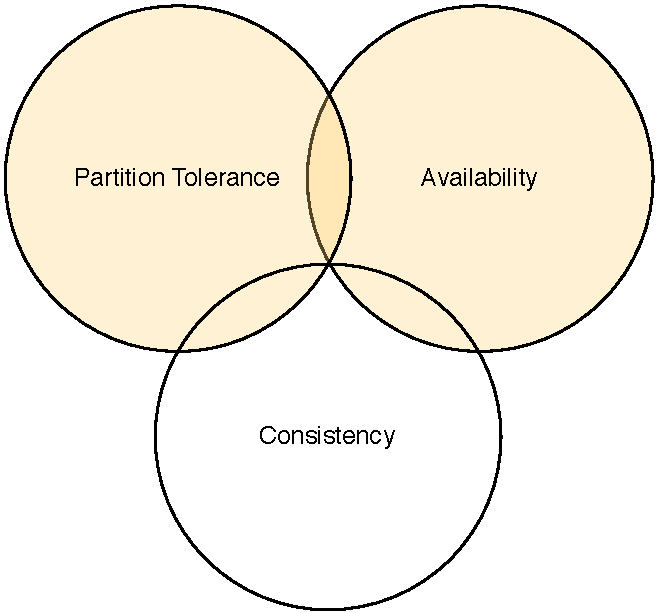
\includegraphics[width=0.5\textwidth]{images/cap}
  \end{center}
  \caption{CAP Theorem}
  \label{fig:cap}
\end{figure}

Eventual consistency means that the storage system guarantees that if no new updates are made to the object, eventually (after the inconsistency window closes) all accesses will return the last updated value. It is seen by many as impracticable for sensitive data, since there is no synchronization that guarantees that updated value will be available at the time of reading. The reality is not so black and white, and the binary opposition between consistent and non consistent is not truly reflected in practice, there are instead degrees of consistency such as strong or causal consistency~\cite{Vogels2008}.

So, on one hand there is the \ac{vlsd} approach, which offers higher scalability, meaning that it can take advantage of having more machines to be able to maintain or even increase its level of performance under bigger loads. On the other hand, a \ac{rdbms} offers more consistency as well as much more powerful query capabilities, leveraging a lot of knowledge and expertise gained over the years \cite{stonebraker2010sql}.  

\section{Problem Statement}

\begin{quote}
If you want to work with a lot of data and be able to run dynamic ad-hoc queries on it, you use a relational database with \ac{sql}. Using a key value store doesn't make any sense for that unless you want to easily be able to distribute your workload on several machines without having to go though the hassle of setting up a relational database cluster. If you want to just keep your objects in a persistent state and have high-performance access to them (e.g. a LOT of web applications), use a key value store.
\end{quote} 
\begin{flushright}in \url{http://buytaert.net/nosql-and-sql}, 25/11/2010\end{flushright}

This separation happens due to the fact that \acp{vlsd} do not provide strong consistency in order to provide partition tolerance and availability, so important in scalable systems. Their reduced \ac{api} makes it simpler and faster to do operations such as a \emph{get} or a \emph{put}. Also, they are prepared from the ground up to replicate data through various machines and even data warehouses.

However, they also have disadvantages as the lack of a standardized query language such as \ac{sql}, making the code vendor specific which in turn makes it less portable. Their simple \ac{api} makes it harder to perform more complex queries and sometimes even impossible since the data is replicated, which makes it hard to maintain an update order and to provide a transactional system with ACID properties. 

These, alongside with the dynamic or non existent schema of these databases, are the main reasons why it is very hard to migrate data and code from a relational database. This kind of migration would save a lot of time and money for companies with huge amounts of code and work done upon relational databases that wish to experience a different type of data storage system.

\section{Objectives}

Migration of data and code is, therefore, something unwanted by developers and managers since it will incur into costs for both, of time and money, respectively. 

According to a blog post by Michael Stonebraker~\cite{stoneEnter}, 61\% of enterprise users are either ignorant about or uninterested in NoSQL\footnote{\acp{vlsd} are subset of NoSQL, since NoSQL does not enforce databases to be distributed}. This happens mainly due to three reasons, because it \textbf{does not provide ACID}, it has a \textbf{low level interface} instead of a high-level language as \ac{sql} and because there is \textbf{no standard} for NoSQL interfaces.

There have been some attempts to make database code the less vendor specific as possible, such as polyglot \acp{orm}\footnote{An orm that outputs different code, according to the database in use, in spite of receiving the same input} as Ruby's DataMapper \cite{DM}, an approach that comes from the fact that even \ac{sql} may differ from \ac{rdbms} to \ac{rdbms} in certain aspects. This portability, however, carries an overhead since it must translate the code to the specific \ac{sql} subset of the required \ac{dbms}.

One problem that \acp{orm} do not solve is migrating legacy \ac{sql} code to a different data model, such as to a \ac{vlsd}. It is exactly this problem that this work aims to tackle, by building a thin layer between the \ac{sql} engine's interpreter and processor, and the actual database underneath it, providing a way to run \ac{sql} queries on top of a \ac{vlsd}.

Alongside with this problem comes another that arise from the limitations of a \ac{vlsd} which is the fact that there is no mechanism to encompass transactions in a \ac{vlsd} and consequently provide the desired ACID properties, which is a problem that this work also addresses and proposes to solve.

To summarize, this work aims:

\begin{itemize}
	\item Allow legacy \ac{sql} code migration to a \ac{vlsd}, taking advantage of a standard language to serve as interface
	\item Provide transactional functionality to the underlying \ac{vlsd}
\end{itemize}

\section{Contributions}

This thesis proposes to provide full \ac{sql} functionality over \ac{vlsd} by altering the \ac{rdbms} underlying storage system.
The major factor in this implementation is that it takes advantage of the scalability and replication features from the \ac{vlsd}, and allies them with the \ac{rdbms} \ac{sql} engine. Also, it provides a completely separate library for transactions in a \ac{vlsd}. 

In detail, we make the following contributions:

\begin{itemize}
	\item \textbf{Prototype database system providing full \ac{sql} functionality over \ac{vlsd}}\\
	   We developed a prototype that allows for \ac{sql} queries to be run over a \ac{vlsd}. In detail, we ported the Apache Derby's query engine to use the Cassandra \ac{vlsd} as its storage layer.
		
	\item \textbf{Distributed transactions library for a \ac{vlsd}}\\
		We developed a library that allows to create and manage transactional contexts enabling to ensure ACID guarantees. 
		
	\item \textbf{Evaluation of the proposed solution}\\
		We evaluate the developed solution using the TPC-W benchmark~\cite{tpcw}, analyzing its behavior under different conditions and configurations comparing its performance to that of a standard \ac{rdbms}. We also evaluated it using the \ac{ycsb} in order to measure the performance of the transactions library without Derby's query engine.
\end{itemize}


\section{Dissertation Outline}

This thesis is organized as follows: Chapter 2 describes the main features of most \acp{vlsd} and some of the implementations; Chapter 3 introduces \ac{sql} and its main functionalities; Chapter 4 describes the modifications made to both Derby and Cassandra in our implementation; Chapter 5 introduces the proposed solution for distributed transactions for \acp{vlsd}; Chapter 6 evaluates the solution implemented using realistic workloads; Chapter 7 describes the related work; and finally Chapter 8 concludes the thesis, summarizing its contributions and describing possible future work. 

		\mbox{}
    \chapter{VLSDs}
        \acp{vlsd} in general provide high availability and elasticity in a distributed environment composed by a set of commodity hardware. This is a whole new paradigm that avoids the need to invest in very powerful and expensive servers to host the database. In addition, these data stores also provide replication, fail-over, load balancing and data distribution. Also, their data model is more flexible than the relational one since the cost of maintaining its normalized data model, by the enforcement of relations integrity, and the ability to run
transactions across all data in the database make it difficult to scale~\cite{Vilaca:2010:ETL:1926129.1926137}. 

Nevertheless, when compared to \acp{rdbms} which have been widely used over the last 30 years and are therefore much more mature, \ac{vlsd} databases have some fundamental limitations that should be taken into account. They provide high scalability at the expense of a more relaxed data consistency model (usually eventual consistency~\cite{Vogels2008}) and only provide primitive querying and searching capability that do not comply to a standard as is the case of \ac{sql} for \acp{rdbms}. Thus, data abstraction and consistency becomes responsibility of the application developers and the code becomes vendor specific.

In this chapter we will introduce some of the most popular \acp{vlsd} and detail Apache's Cassandra in particular since it was the one we chose to develop our work upon.

\section{Project Voldemort}
Voldemort is an eventually consistent key-value store~\cite{nosqlOrg} written in Java and is an open source implementation of Amazon's Dynamo~\cite{Hastorun2007}. As such, each node is independent of other nodes with no central point of failure or coordination. It is used  at LinkedIn for certain high-scalability storage problems where simple functional partitioning is not sufficient~\cite{voldemort}.

\subsubsection{Data Storage}

Voldemort has a very simple \ac{api} and supports pluggable serialization to allow for rich keys and values to integrate with serialization frameworks like Protocol Buffers, Thrift, Avro, Java Serialization and JSON. 

Also, in order to make the system more resilient to server failure data is replicated through N servers, which means it tolerates up to N-1 failures without losing data. To mitigate the problems that arise with replication, such as multiple updates on different server or a server not being aware of an update do to a crash, Voldemort uses data versioning with vector clocks~\cite{fidge_vector_clocks_1988} that resolve inconsistencies at read time. 

Voldemort's cluster may serve multiple stores and each of them has a unique key space and storage definition, such as serialization method or the storage engine used\footnote{the underlying storage used by Voldemort can be the BerkeleyDB JE, MySQL or read-only stores, others may be used, since it is pluggable}.

\subsubsection{Clustering and Replication}

The request routing in Voldemort is done with consistent hashing\footnote{``Consistent hashing is a scheme that provides hash table functionality in a way that the addition or removal of one slot does not significantly change the mapping of keys to slots. By using consistent hashing, only K/n keys need to be remapped on average, where K is the number of keys, and n is the number of slots.'' in Wikipedia, 13/12/2010}) which assigns nodes to multiple places on the hash ring providing automatic load balance and ability to migrate partitions.

Voldemort provides eventual consistency and as such it focuses on the A (availability) and P (partition tolerance) of the CAP theorem. This trade-off between consistency and availability can be tuned by the client since each of the data stores can have a different number of nodes to which data is replicated, the \textbf{N} value or preference list, and the values \textbf{R} and \textbf{W} for quorum reads and writes, respectively. When reading data, it will read from the first R available replicas in the preference list, return the latest version and repair the obsolete ones. If causality can’t be determined, client side reconciliation is allowed. When writing in quorum, the update is done synchronously for W replicas in the preference list and asynchronously to the others.  

This leads to the inequality \ref{eq:ineq} that provides read-your-writes consistency which is the stronger consistency available.

\begin{equation}
	R + W > N
\label{eq:ineq}	
\end{equation}	

\section{Riak}

Riak is a key-value store~\cite{nosqlOrg} written mostly in Erlang and C, developed by Basho Technologies and is, according to them~\cite{riakWeb}, heavily influenced by the CAP theorem and Amazon's Dynamo paper~\cite{Hastorun2007}. It is master-less, i.e. all nodes in a Riak cluster are equal, each node is fully capable of serving any client request which means that there is no single point of failure. 

\subsubsection{Data Storage}

Riak structures data using buckets, keys and values, being that the values are referenced by a unique key and each key value pair is stored in a bucket. Thus, buckets provide different namespaces making it possible for the keys with the same name to coexist in a Riak cluster.

Its \ac{api} uses \ac{rest} and the storage operations use \ac{http} PUTs and POSTs and fetches use \ac{http} GETs which are submitted to a predefined \ac{url} (default is ``/riak''). In order to take full advantage of this Riak also provides a functionality called links, that are are metadata that establish one-way relationships between objects in Riak and can be used to loosely model graph like relationships between them.

\subsubsection{Clustering and Replication}

Physical servers, referred to in the cluster as \textbf{nodes}, run a certain number of virtual nodes, or \textbf{vnodes}. Each vnode will claim a partition on the ring and the number of active vnodes per node is determined by the number of physical nodes in the a cluster at any given time. 

Each node in the cluster is responsible for 1/(total number of physical nodes) of the ring and the number of vnodes of each node can be determined by calculating (number of partitions)/(number of nodes). As an example consider a ring with 32 partitions, composed of four physical nodes, it will have approximately eight vnodes per node.

Riak's bucket information is communicated across the cluster through a gossip protocol, this includes the \emph{hinted handoff} mechanism used to compensate for failed nodes, in which the failed node neighbors will perform its work, allowing for the cluster to continue to work.  

The number of nodes to which data is replicate, the \textbf{N} value, is defined in a per bucket basis, but all nodes in the same cluster should agree and use the same N value. When reading or writing data, Riak allows the client to supply a value, \textbf{R} and \textbf{W} respectively, that represents the number of nodes which must return results in order for a read or write to be considered successful. 

Since multiple updates can occurs in different nodes, there has to be a way to reconcile an arrive to a mutual consistent state for the system. To do that, this system uses vector clocks to keep track of at what version each object is. More specifically, by looking at two vector clock Riak must determine whether one object is a direct descendant of the other, the objects are direct descendants of a common parent or if the objects are unrelated in recent heritage. With this information it can then proceed to auto-repair data that is out of sync or at least provide the client with an opportunity to reconcile them in an application specific manner. 

Since it first major release Riak adds the support for Secondary Indexes, allowing an application to tag a Riak object with one or more field/value pairs. The object is indexed under these field/value pairs, and the application can later query the index to retrieve a list of matching keys.

\section{Apache HBase}
HBase is a wide column store~\cite{nosqlOrg} modeled after Google's BigTable~\cite{Chang2008} and is written in Java. It is developed as part of Apache Haddop\footnote{\url{http://hadoop.apache.org/}} project providing a fault-tolerant way of storing large quantities of sparse data while providing strong consistency. 

\subsubsection{Data Storage}
HBase stores its data in tables which are composed of rows and columns, being that each column must belong to a specific column family. The row keys are stored in byte-lexicographical order since they are raw byte arrays instead of strings, furthermore within a row the columns are stored in a sorted order.

Each column is versioned and HBase can store multiple version of every cell and does so in decreasing order so that the most recent values are found first, when reading from a store file. This means that when insert or updating a column, the client must specify its name, value and timestamp. 

\subsubsection{Clustering and Replication}
An HBase cluster is composed by a Master node, responsible for telling the clients in which region server to look for the data, multiple region servers, that are responsible for several regions (parts) of the data of the whole cluster. Each region has a log to whom the changes written to before they are actually pushed to disk, this log is then replicated to a distributed file system, Apache's \emph{HDFS}.

This system also depends on running a ZooKeeper cluster that is used to store membership information, which allows to detect dead servers and to perform master election and recovery from failures. For instance the master can be killed and the cluster will continue to function, by finding a new master.

\section{Cassandra}
\label{sec:cassandra}
Cassandra~\cite{will10}, that was created on Facebook, first started as an incubation project at Apache in January of 2009 and is based on Dynamo~\cite{Hastorun2007} and BigTable~\cite{Chang2008}. This system can be defined as an open source, distributed, decentralized, elastically scalable, highly available, fault-tolerant, tuneably consistent, column-oriented database~\cite{hewitt2010cassandra}. 

Cassandra is distributed, which means that it is capable of running on multiple machines while the users see it as if it was running in only one. More than that, Cassandra is built and optimized to run in more than one machine. So much that you cannot take full advantage of all of its features without doing so. In Cassandra, all of the nodes are identical, there is no such thing as a node that is responsible for certain organizing operations, as in BigTable or HBase. Instead, Cassandra features a peer-to-peer protocol and uses gossip to maintain and keep in sync a list of nodes that are alive or dead. 

Being decentralized means that there is no single point of failure, because all the servers are symmetrical. The main advantages of decentralization are that it is easier to use than master/slave and it helps to avoid suspension in service, thus supporting high availability.

Scalability is the ability to have little degradation in performance when facing a greater number of requests. It can be of two types:

\begin{description}
	\item[Vertical] Adding hardware capacity and/or memory
	\item[Horizontal] Adding more machines with all or some of the data so that all of it is replicated at least in two machines. The software must keep all the machines in sync. 
\end{description}

Elastic scalability refers to the capability of a cluster to seamlessly accept new nodes or removing them without any need to change the queries, rebalance data manually or restart the system.

Cassandra is highly available in the sense that if a node fails it can be replaced with no downtime and the data can be replicated through data centers to prevent that same downtime in the case of one of them experiencing a catastrophe, such as an earthquake or flood. 

Consistency essentially means that a read always return the most recently written value, which is guaranteed to happen when the state of a write is consistent among all nodes that have that data (the updates have a global order). Most \acp{vlsd}, including Cassandra, focus on availability and partition tolerance, relaxing the consistency guarantee, providing eventual consistency.  

In the particular case of Cassandra consistency can be considered tuneable in the sense that the number of replicas that will block on an update can be configured on an operation basis by setting the consistency level combined with the replication factor (Section \ref{sec:consistency}).


\subsection{Data Model}
\label{sec:cass_data_model}
Cassandra is a row oriented\footnote{It is frequently referred to as column oriented, but data in Cassandra is actually stored in rows indexed by a unique key, but each row does not need to have the same columns (number or type) as the ones in the same column family.} database system, with a rather complex data model~\cite{sarkissian09}, that is described below.

The basic building block of Cassandra are columns (Fig. \ref{fig:column}) that consist of a tuple with three elements, a name, a value and a timestamp. The name of column can be a string but, unlike its relational counterpart, can also be long integers, UUIDs or any kind of byte array.

\begin{figure}[htb]
  \begin{center}
    \leavevmode
    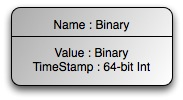
\includegraphics[width=0.3\textwidth]{images/column.jpg}
  \end{center}
  \caption{Cassandra Column}
  \label{fig:column}
\end{figure}

Sets of columns are organized in rows that are referenced by a unique key, the row key, as demonstrated in figure \ref{fig:row}. A row can have any number of columns that are relevant, there is no schema binding it to a predefined structure. Rows have a very important feature, that is that every operation under a single row key is atomic per replica, despite the number of columns affected. This is the only concurrency control mechanism provided by Cassandra.

\begin{figure}[!htb]
  \begin{center}
    \leavevmode
    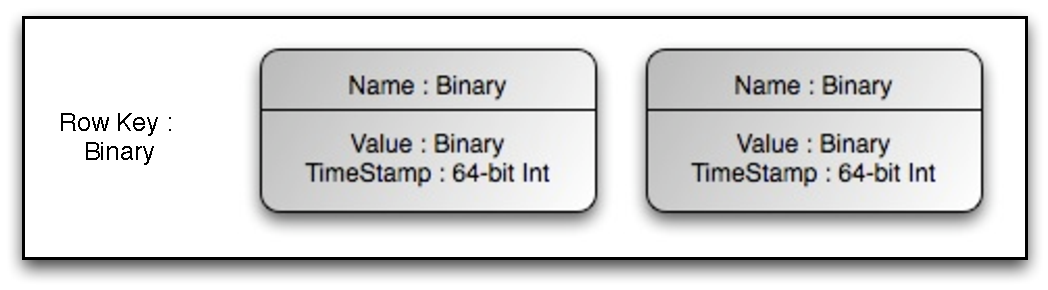
\includegraphics[width=0.8\textwidth]{images/row}
  \end{center}
  \caption{Cassandra Row}
  \label{fig:row}
\end{figure}

The maximum level of complexity is achieved with the column families, which ``glue'' this whole system together, it is a structure that can keep an infinite\footnote{Limited by physical storage space} number of rows, has a name and a map of keys to rows as shown in picture \ref{fig:columnfamily}. 

Applications can specify the sort order of columns within a column family, based on their name, and order them by its value in bytes, converted to an integer or a string, or even as a 16-byte timestamp.

\begin{figure}[!htb]
  \begin{center}
    \leavevmode
    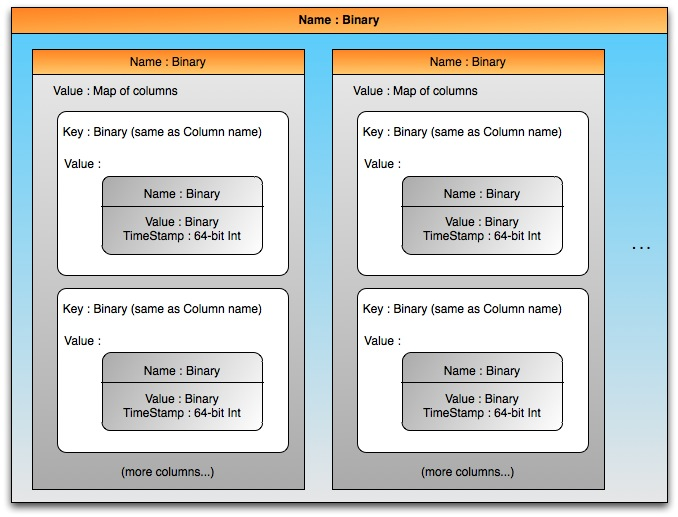
\includegraphics[width=0.8\textwidth]{images/columnfamily}
  \end{center}
  \caption{Cassandra ColumnFamily}
  \label{fig:columnfamily}
\end{figure}


Cassandra also provides another dimension to columns, the SuperColumns (Fig. \ref{fig:supercolumn}), these are also tuples, but only have two elements, the name and the value. The value has the particularity of being a map of keys to columns (the key has to be the same as the column's name).

\begin{figure}[htb]
  \begin{center}
    \leavevmode
    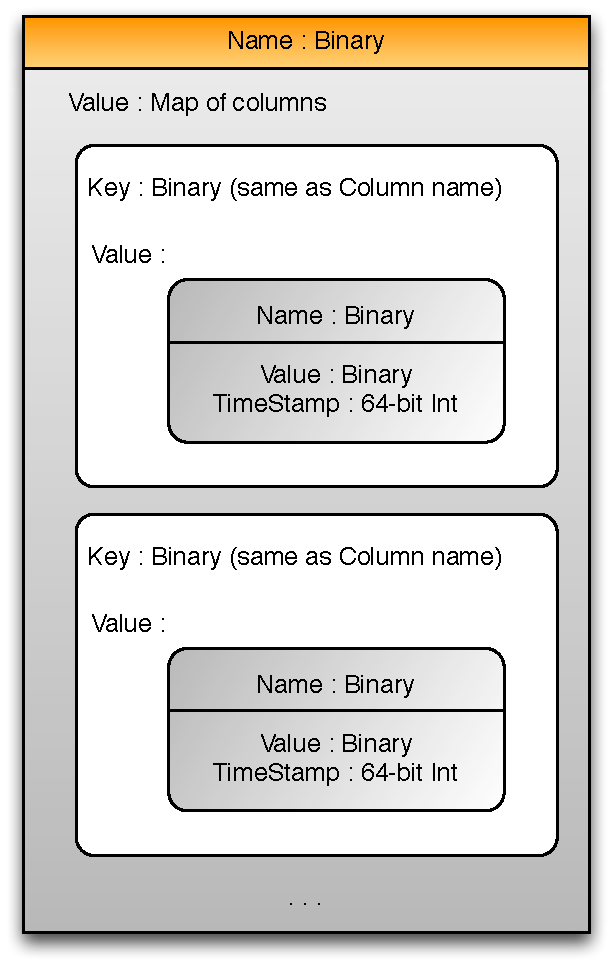
\includegraphics[width=0.4\textwidth]{images/supercolumn}
  \end{center}
  \caption{Cassandra SuperColumn}
  \label{fig:supercolumn}
\end{figure}

There is a variation of ColumnFamilies that are SuperColumnFamilies. The only difference is that where a ColumnFamily has a collection of name/value pairs, a SuperColumnFamily has subcolumns (named groups of columns). This is better understood by looking at the path a query takes until reaching the desired value in both a normal and super column family (Table \ref{tab:path}).

\begin{table}[h!]
\centering
  \begin{tabular}{@{}p{4cm}  r@{}}
	\toprule
	\textbf{Normal} & $Row key \rightarrow Column name \rightarrow Value$\\
    \textbf{Super}  & $Row key \rightarrow Column name \rightarrow Subcolumn name \rightarrow Value$\\
    \bottomrule
  \end{tabular}

\caption{Path to get to value}
\label{tab:path}
\end{table}

Multiple column families can coexist in an outer container called keyspace. The system allows for multiple keyspaces, but most of deployments have only one.

\subsubsection{Partitioners}
\label{sec:partitioners}

Partitioners define the way rows are ordered in Cassandra. By default the one used is the Random partitioner that combines MD5 hashes of the keys with consistent hashing to determine the place where these keys belong in the ring (Section \ref{sec:consistency}). This spreads the keys evenly trough the ring due to its random distribution, but also makes it very inefficient\footnote{most of the times a range query would imply returning the whole set of keys, and filter it.} to perform (even impossible to do from the Cassandra client). 

Since our work relies largely on performing range queries on keys composed of byte arrays, the partitioner used is the Byte-Ordered Partitioner. It is an Order-Perserving Partioner\footnote{Rows are stored by key order, aligning the physical structure of the data with that order} that treats the data as raw bytes, instead of converting it to strings.    


\subsection{Querying}
Cassandra's \ac{api} defines its querying capabilities, and consists of three simple methods\footnote{The actual client API has more methods that are variations of these or schema related}~\cite{lakshmanMalik}:

\begin{itemize}
	\item \emph{insert(table, key, rowMutation)}
	\item \emph{get(table, key, columnName)}
	\item \emph{delete(table, key, columnName)}
\end{itemize}	

In the method signatures above, \emph{columnName} can refer to a specific column in a column family, a column family, normal or super, or a column in a supercolumn. The \emph{rowMutation} specifies the changes to the row in case it was already there, or the row to be added\footnote{Cassandra treats updates as inserts to existent rows, that is the reason there is no update operation}, Mutations can also be Deletions that represent deletes when performing a batch insert.

\subsection{Consistency}
\label{sec:consistency}
Cassandra allows clients to specify the desired consistency level on reads and writes, based on the replication factor previously defined in a configuration file, present in every cluster. Notice that if the inequality \ref{eq:ineq} holds, for R as the number of nodes to block for on read, and W the ones to block for on write, the most consistent behavior will be achieved\footnote{Because the replication process only requires a write to reach a single node to propagate, a write which ``fails'' to meet consistency requirements will still appear eventually as long as it was written to at least one node.}. Obviously his affects the performance and availability, since all update operations must wait for the update to occur in every node.

Cassandra uses replication to achieve high availability and durability. Each data item is replicated at N nodes, where N is the afore mentioned replication factor, assigning each key to a coordinator node (chosen through consistent hashing, that in addition to storing locally each key within his range, replicates these keys at the N-1 nodes in the consistent hashing ring. 

Cassandra system elects a leader amongst its nodes using Zookeeper~\cite{Junqueira2007}, that is contacted by all joining nodes, and tells them for what ranges they are responsible. The leader also makes an effort for maintaining the invariant that no node is responsible for more than N-1 ranges in the ring. 

In Cassandra every node is aware of every other node in the system and, therefore the range they are responsible for.




   	    \mbox{}		
    \chapter{SQL}
       \ac{sql} is the most widely accepted and implemented interface language for relational database systems, and it was one of the first commercial languages for Edgar F. Codd's relational model~\cite{codd1970relational}. Originally based upon relational algebra and tuple relational calculus, its scope includes data insert, query, update and delete, schema creation and modification, and data access control.

The database world being so integrated boosts the importance of a standard language that can be used to operate in many different kinds of computer environments and on many different \acp{dbms}~\cite{Gruber:2000:MS:518858}. A standard language allows you to learn one set of commands and use it to create, retrieve, alter, and transfer information regardless of whether you are working on a personal computer or a workstation. It also enables you to write applications that access multiple databases, as applications that use the ODBC \ac{api}.

The \ac{sql} standard is defined jointly by \ac{ansi} and \ac{iso} that have published a series of \ac{sql} standards since 1986, each being a superset of its predecessor. These standards tend to be ahead of the industry by several years, in the sense that many products today still conform to SQL99.

In a sense, there are three forms of \ac{sql}, Interactive, Static and Dynamic. For the most part they operate the same way, but are used differently.

\begin{description}
	\item[Interactive \ac{sql}] Used to operate directly on a database to produce immediate output for human utilization
	\item[Static \ac{sql}] Consists of \ac{sql} statements hard-coded as part of an application. The most common form of this is \emph{Embedded \ac{sql}}, where the code is infixed into the source code of a program written in another language. This requires some extensions to Interactive \ac{sql} as the output of the statements must be ``passed of'' to variables or parameters usable by the program in which it is embedded.
	\item[Dynamic \ac{sql}] Also part of an application, but the \ac{sql} code is generated at runtime. 
\end{description}

This chapter will further explain the \ac{sql} concepts that are necessary in order to fully understand our work.

\section{SQL Statements}

\emph{Statements}, or commands, are instructions you give to an \ac{sql} database and consist of one or more logically distinct parts called \emph{clauses}. Clauses generally begin with a keyword for which they are named and consist of other keywords and arguments. Examples of a clauses could be \emph{FROM TUPLEitem} and \emph{WHERE i\_id = 1589}. Arguments complete or modify the meaning of a clause. In the previous examples, \emph{TUPLEitem} is the argument and \emph{FROM} is the keyword of the \emph{FROM} clause. Likewise \emph{i\_id = 1589} is the argument of the \emph{WHERE} clause.

\subsection{Create}

In order to create the above mentioned \emph{TUPLEitem} table you would use the \emph{CREATE TABLE} statement, code sample \ref{lst:create_item}.

\lstset{
  language=SQL, 
  caption=SQL create table statement, 
  label=lst:create_item,
}
\definecolor{shadecolor}{gray}{0.95}


\begin{shaded}
\begin{lstlisting}
CREATE TABLE TUPLEitem 
   ( i_id      int            not null, 
     i_title   varchar(60),
     i_stock   int, 
     i_isbn    char(13),
     PRIMARY KEY(i_id));
\end{lstlisting}  
\end{shaded}  

This statement has the following components:
\begin{itemize}
	\item \emph{CREATE TABLE} are the keywords indicating what this statement does
	\item \emph{TUPLEItem} is the name given to the table
	\item The items in parenthesis are a list of the columns in the table. Each column must have a name and a datatype. It may also have one or more constraints as \emph{not null} or \emph{primary key}
\end{itemize}

Note that this statement makes some assumptions such as the fact that the primary key for each row is not defined by default, it must be explicitly declared. It is, however, highly advised to define one and therefore we shall assume from this point on that each table has a primary key composed of one or more of its columns. When it is defined, an index is created for the values used as primary key which is used when retrieving it. The statement also assumes that a value can be null.

\subsection{Insert}
\label{sec:sql_insert}

The created table does not yet contain data, to insert a row into the table you would use the statement with the self-explaining name \emph{INSERT} (code sample \ref{lst:insert_item}). If there is already a row with the same primary key as the one being inserted, an error should be raised and no changes made to the database. 

\lstset{
  language=SQL, 
  caption=SQL insert statement, 
  label=lst:insert_item,
}
\definecolor{shadecolor}{gray}{0.95}


\begin{shaded}
\begin{lstlisting}
INSERT INTO TUPLEItem VALUES 
         (100,'Nice title',10,'0782125387');
\end{lstlisting}  
\end{shaded}

This inserts the list of values in parentheses into the \emph{TUPLEItem} table, with the particularity that the values are inserted in the same order as the columns into which they are being inserted and that the text data values are enclosed in single quotes. 

Also note that the table name must have been previously defined in a \emph{CREATE TABLE} statement and that each value enumerated in the \emph{VALUES} clause must match the datatype of the column into which it is being inserted, with the exception of \emph{NULL} values, which are special markers to represent values that you do not possess information for, and can be inserted into any datatype as long as the column allows them.

\subsection{Update}
In order to change some or all of the values in an existing row there is the \emph{UPDATE} statement which is composed by two parts, the \emph{UPDATE} clause that names the table affected and a \emph{SET} clause that indicates the change(s) to be made to certain column(s). For instance, if you want to increment the stock for the item inserted in section \ref{sec:sql_insert} you would do the following:

\lstset{
  language=SQL, 
  caption=SQL update statement, 
  label=lst:update_item,
}
\definecolor{shadecolor}{gray}{0.95}


\begin{shaded}
\begin{lstlisting}
UPDATE TUPLEItem
     SET i_stock = i_stock + 1 
     WHERE i_id = 100
\end{lstlisting}  
\end{shaded}

It is possible to use value expressions in the \emph{SET} clause including expressions that employ the column being modified, as the increment of the stock by one in the example above. Whenever you refer to an existing column value in this clause, the value produced will be that of the current row before the \emph{UPDATE} makes any changes.

Also, in order to update only one of the rows instead of all the rows in the table the \emph{WHERE} clause is used.

\subsubsection{Where}
\label{sec:sql_where}

Tables tend to get very large and most of the times you do not wish for your statements to affect all of the rows in a certain table. This is the reason why \ac{sql} enables you to define criteria to determine which rows to select and this is achieved using \emph{WHERE}, which allows you to define a condition that may evaluate to \emph{TRUE}, \emph{FALSE} or \emph{UNKNOWN}. All the rows that are being evaluated are called \textbf{candidate rows} and of those, the ones that make the predicate \emph{TRUE} are called \textbf{selected rows}, and obviously are the ones retrieved to the client. In order to do this, the database manager must go through the entire table one row at a time and examine it to evaluate if the predicate is true.  

There are many operators that can be used in predicates, in the previous example we used the $=$ operator but other inequalities as $<$ (less than), $>$ (greater than) or $<>$ (not equal to) also apply. The standard boolean operators \emph{NOT}, \emph{AND} and \emph{OR} also apply and can be used to concatenate various predicates or to deny the result of one in the case of \emph{NOT}.

This operators differ from most programming languages in the special case of finding a \emph{NULL} value in the column being evaluated. As aforementioned \ac{sql} boolean expressions can evaluate to three values instead of the usual two, the extra value is \emph{UNKNOWN}, which is used for that special case. If you do not take this differences into account, it might change the way the statement behaves. The main differences between two and three-valued logic are illustrated in Table \ref{tab:logic_diff}.

\renewcommand\arraystretch{2.0}
\begin{table}[h!]
\centering
  \begin{tabular}{  m{6cm}  m{4cm} }
	\toprule
	\textbf{Predicate} & \textbf{Truth Value}\\
    \midrule
    \emph{NOT UNKNOWN} & \emph{UNKNOWN}\\
    %\hline
    \emph{TRUE OR UNKNOWN} & \emph{TRUE}\\
    %\hline
    \emph{FALSE OR UNKNOWN} & \emph{UNKNOWN}\\
    %\hline
    \emph{TRUE AND UNKNOWN} & \emph{UNKNOWN}\\
    %\hline
    \emph{FALSE AND UNKNOWN} & \emph{FALSE}\\
    \bottomrule
  \end{tabular}

\caption{Three-valued logic main differences}
\label{tab:logic_diff}
\end{table}

Regarding \ac{sql} predicates there are some things of note. Firstly, as just mentioned, it allows for \emph{NULL} values to be stored as a value of any type and therefore to be evaluated as such, using the three-valued logic. Secondly, with the composition of inequalities, it allows to do range queries, i.e. queries that encompass all the rows with id from 1 to 10, for example.

\subsection{Select}
A query is a statement you give to the \ac{dbms} that tells it to produce certain specified information~\cite{Gruber:2000:MS:518858}. In \ac{sql} all queries are constructed from a single statement that can be extended to allow some highly sophisticated evaluating of data. This statement is \emph{SELECT}.

In its simplest form, it instructs the database to retrieve the contents of a table. For instance, you could retrieve all the rows in the \emph{TUPLEItem} table with the following statement:

\lstset{
  language=SQL, 
  caption=SQL select statement, 
  label=lst:select_item,
}
\definecolor{shadecolor}{gray}{0.95}


\begin{shaded}
\begin{lstlisting}
SELECT * FROM TUPLEItem;
\end{lstlisting}  
\end{shaded}  

The statement is pretty much self explaining, with the exception of \emph{*} which is a wildcard that expands to all of the columns in the row\footnote{As globbing in \emph{BASH}}. Therefore the statement \textbf{selects} all the columns in the row \textbf{from} each row of the table \textbf{TUPLEItem}.

If you want to select certain columns instead of all, just switch \emph{*} for a comma separated list of column names.

This will, however, return what is know in mathematical terms as a multiset (or bag), i.e. a collection in which member are allowed to appear more than once. In order to retrieve an actual mathematical set, i.e. a collection of distinct values, you can use the argument called \emph{DISTINCT} in conjunction with the \emph{SELECT} statement as shown in code sample \ref{lst:select_distinct_item}.

\lstset{
  language=SQL, 
  caption=SQL select distinct statement, 
  label=lst:select_distinct_item,
}
\definecolor{shadecolor}{gray}{0.95}


\begin{shaded}
\begin{lstlisting}
SELECT DISTINCT i_title FROM TUPLEItem;
\end{lstlisting}  
\end{shaded}  

Querying gains much more expressiveness and power when used together with the where clause in the exact same way as the \emph{UPDATE}, as explained in Section \ref{sec:sql_where}. It also takes implicit advantage of indexes, since the \ac{dbms} will optimize the retrieval of the data and use indexes in those cases where it believes it is better (faster) to do so.

\subsection{Delete}

Rows can be deleted from a table with the \emph{DELETE} statement and since only entire rows can be deleted, no column argument is accepted. Code sample \ref{lst:delete_item} will remove all the contents in \emph{TUPLEItem}.

\lstset{
  language=SQL, 
  caption=SQL delete statement, 
  label=lst:delete_item,
}
\definecolor{shadecolor}{gray}{0.95}

\begin{shaded}
\begin{lstlisting}
DELETE FROM TUPLEItem;
\end{lstlisting}  
\end{shaded}

As most \ac{sql} statements that affect rows, \emph{DELETE} can be used with \emph{WHERE}, in order to delete specific rows instead of all of them.

This statement can only be used to delete rows, if you want to delete a table you must execute a two step process. First you must empty the table of any data with the \emph{DELETE} statement and then destroy the definition of the table with the \emph{DROP} statement. 

\lstset{
  language=SQL, 
  caption=SQL drop statement, 
  label=lst:drop_item,
}
\definecolor{shadecolor}{gray}{0.95}

\begin{shaded}
\begin{lstlisting}
DROP TABLE TUPLEItem;
\end{lstlisting}  
\end{shaded}

\section{Special Operators}

Other than the relational and boolean operators \ac{sql} also provides a set of special operators that can be used to produce more sophisticated and powerful predicates. 

\subsection{In}
The \emph{IN} operator explicitly defines a set in which a given value may or may not be included. It defines the set by naming the members in parentheses separated by commas, and then tries to match the column value of the row being tested with any of the values in the set. If it finds one, the predicate is \emph{TRUE}.

\subsection{Between}

The \emph{BETWEEN} operator is similar to \emph{IN}, but rather than enumerating a set it defines a range that values must fall into in order to make the predicate \emph{TRUE}. The keyword \emph{BETWEEN} is followed by the start value, the keyword \emph{AND} and the end value, with the particularity that the first value must appear first in alphabetic or numeric order than the last (unlike \emph{IN}, where order does not matter).

Also, the range is inclusive by default and \ac{sql} does not directly support a noninclusive \emph{BETWEEN}.  

\subsection{Like}

The \emph{LIKE} operator is used with text string datatypes only and is used to find substrings in them, i.e. it searches a text column to see if part of it matches a given string. In order to do this, it uses two types of wildcards:

\begin{itemize}
	\item $\textunderscore$ stands for any single character, it corresponds to \emph{.} in \emph{Regex}.
	\item $\%$ stands for a sequence of any number of characters, including zero, the corresponding to \emph{.*} in \emph{Regex}
\end{itemize} 

\lstset{
  language=SQL, 
  caption=SQL like operator, 
  label=lst:like_item,
}
\definecolor{shadecolor}{gray}{0.95}

\begin{shaded}
\begin{lstlisting}
SELECT * FROM TUPLEItem
     WHERE i_title LIKE 'N__e t%' 
\end{lstlisting}  
\end{shaded}

In code sample \ref{lst:like_item}, the predicate will match any item in the table \emph{TUPLEItem} that has a title that starts with the letter \emph{N}, has two characters and the an \emph{e} (such as ``Nice'' from our example) and has a second word that starts with a \emph{t} (such as ``title''). Note that it can have other words after the second one, since the $\%$ wildcard will stand for any number of characters until the end of the string.

\subsection{Is Null}
As previously discussed, when a \emph{NULL} is compared to any value (even another \emph{NULL}) the result is \emph{UNKNOWN}. Therefore, if you need to distinguish between a \emph{FALSE} and an \emph{UNKNOWN}, i.e. rows containing values that fail a predicate condition and those containing \emph{NULL}s, \ac{sql} provides the special operator \emph{IS} which is used with the keyword \emph{NULL} to locate and treat \emph{NULL} values.

This can be further enhanced by adding the keyword \emph{NOT}, providing the \emph{IS NOT NULL} operator which is the exact opposite of \emph{IS NULL}. 

\section{Stored Procedures}
\label{sec:stored_procedures}
One of the important extensions provided by \ac{sql} is the ability to invoke routines written in other languages such as C or Java, from \ac{sql}. The way it is done is by specifying routines as \ac{sql} objects that are essentially wrappers for routines written in other languages, and thus providing an \ac{sql} interface to that routine. 

These routines can be either functions, procedures or methods and the difference between them is that functions return a value whereas procedures simply do something (such as a \emph{void} method in Java) and methods return a value that is an actual \ac{sql} object\footnote{SQL objects are schemas, data dictionaries, journals, catalogs, tables, aliases, views, indexes, constraints, triggers, sequences, stored procedures, user-defined functions, user-defined types, and SQL packages~\cite{ibmSql}.}.

In a \ac{dbms}, a stored procedure is a set of \ac{sql} statements with an assigned name that's stored in the database in compiled form so that it can be shared by a number of programs. It has a great number of optional values at the moment of creation, the following example (Code sample \ref{lst:sql_procedure}) shows how to create a stored procedure for an external Java method.

\lstset{
  language=SQL, 
  caption=SQL procedure creation, 
  label=lst:sql_procedure,
}
\definecolor{shadecolor}{gray}{0.95}

\begin{shaded}
\begin{lstlisting}
CREATE PROCEDURE ADDTABLESTOLOCK(TABLES VARCHAR(32672)) 
     PARAMETER STYLE JAVA 
     LANGUAGE JAVA NO SQL 
     EXTERNAL NAME 'cassandraTrans.TransactionInitializer.setTablesToLock'";
\end{lstlisting}  
\end{shaded}

The procedure is executed in response to an explicit statement in the program on behalf of which it is used, that statement is typically know as \emph{call statement}~\cite{Melton:2002:ASU:863098}. A \emph{CALL} statement (Code sample \ref{lst:sql_procedure_invoke}) causes an \ac{sql}-invoked procedure to be invoked and all the information that is transferred to it is passed through its parameters.

\lstset{
  language=SQL, 
  caption=SQL invoking a procedure, 
  label=lst:sql_procedure_invoke,
}
\definecolor{shadecolor}{gray}{0.95}

\begin{shaded}
\begin{lstlisting}
call ADDTABLESTOLOCK('Lock1,Lock2');
\end{lstlisting}  
\end{shaded}

 

   	   \mbox{}
	\chapter{SQL over a VLSD}
	\label{chap:cass}
       Our work focuses on providing the benefits of having a standard and matured language as \ac{sql} to serve as querying interface for a \ac{vlsd}. First we needed a query engine, which is the primary interface to the storage engine and uses \ac{sql} as query language. Generally a query engine is composed by two main stages, the compilation and the execution of the query, being that the first is the one in which most optimizations and the choosing of which algorithms to use according to the estimate cost of each operation take place. The second phase is responsible for the actual implementation of algorithms that manipulate the data of the database, such as the scanning of relations which is essential to access the tuples of a relation, and it can be of three types\footnote{These definitions came from conversation with Francisco Cruz}:

\begin{description}
	\item[Table-scan] Reads each block holding the tuples of a relation
	\item[Index-scan] If there is an index on the table it may be used to retrieve the tuples of a relation 
	\item[Sort-scan] Takes as a parameter the sorting attributes, and produces the result in the desired order
\end{description}

The implementation of the algorithms is where most of our work lies, providing a separating layer from the query engine to the underlying storage engine.

As a query engine we chose Apache DerbyDB which is a full fledged open-source Java \ac{rdbms}, that has a very small footprint\footnote{about 2.6MB of disk-space for the base engine and embedded \ac{jdbc} driver~\cite{derbySite}}.

To store the data we chose the \ac{vlsd} Apache Cassandra that was detailed in section \ref{sec:cassandra}.

\begin{figure}[!ht]
  \begin{center}
    \leavevmode
    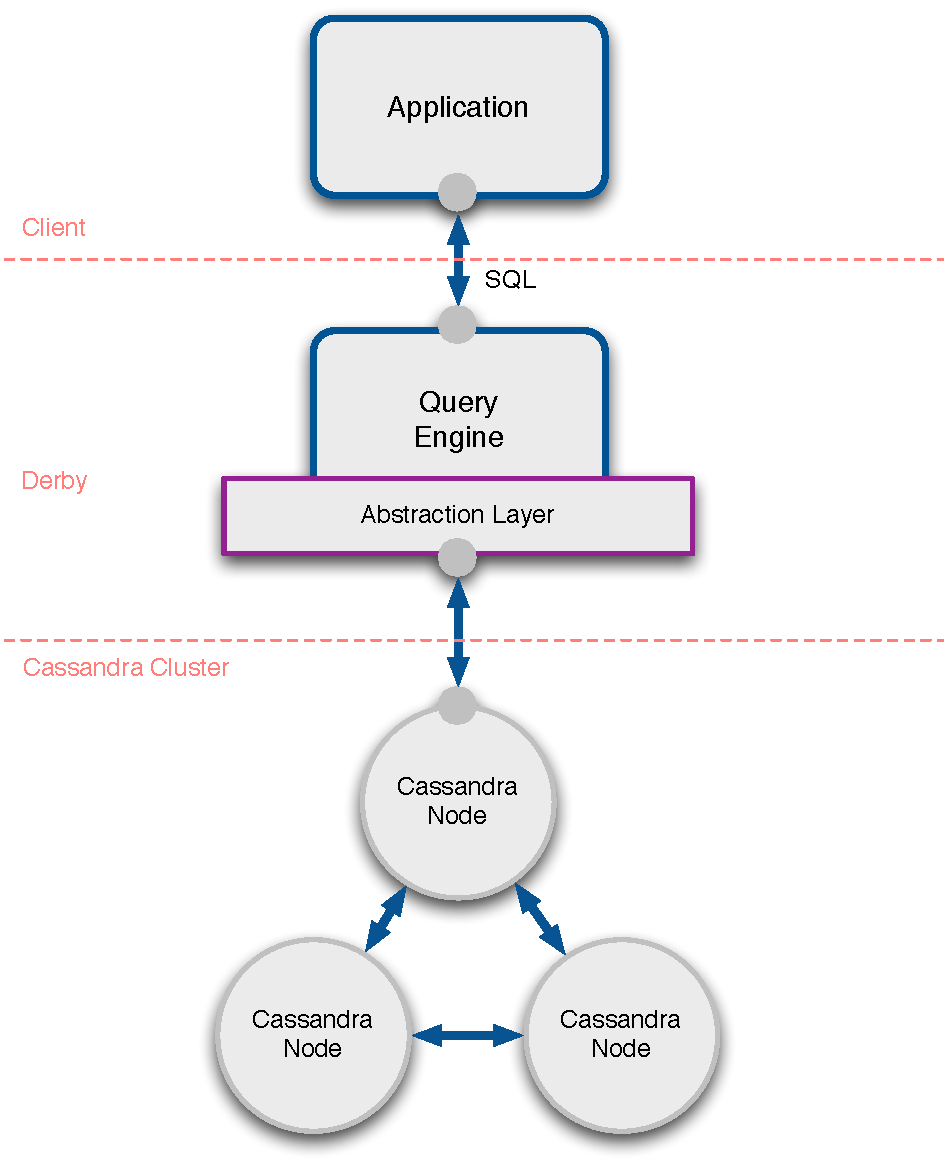
\includegraphics[width=0.9\textwidth]{images/arch}
  \end{center}
  \caption{Derby over Cassandra system architecture}
  \label{fig:derbyCassandra}
\end{figure}

The system architecture is shown in figure \ref{fig:derbyCassandra} and it encompasses an application that has an \ac{sql} interface with the query engine, in this case Derby, which then transfers control to our abstraction layer that will randomly choose a cassandra node from to cluster, connect to it and perform the desired operations. This chapter will focus on the abstraction layer and how it translates the requests into Cassandra's methods.


\section{Abstraction Layer}

The implementation of the abstraction layer involved integrating Derby with Cassandra. On the Derby side this meant changing the way the algorithms are implemented in the storage engine, on Cassandra's side this meant doing two things, defining the way data will be stored and translating Derby operations to its API.  

\subsection{Derby}
\label{sec:patch}

As described above our work prime emphasis is on Derby's storage engine, therefore, before explaining the modifications made there is a need to understand its basic structure.

The Derby engine is composed by multiple packages from which we will focus mainly on the one called \emph{store}, that as the name may suggest is the responsible for the implementation of the storage engine algorithms. Within it lies another package, called \emph{access}, with the specific implementation of said algorithms for each kind of storage\footnote{BTree and Heap are the default ways for interacting with storage in the vanilla Derby}. As would be expected, we wrote similar packages within the access that, when the table name starts with \textbf{TUPLE} (this is our convention), use Cassandra as storage engine. We have named these packages \emph{tuplestore} and \emph{tuplestoreindex} for, respectively, the operations with regular records and with indexes.    

Following Derby's implementation, each type of action has a responsible class, such as the TupleStore for the creation and deletion of tables, the TupleStoreController for insertion, update or deletion of rows and the TupleStoreScanController for fetches that need some sort of scanning. The same applies to index, but the with the suffix Index.

When developing this layer some optimizations were made such as the reutilization of connections, since Derby creates one physical connection to the underlying database for each transaction this can mean a reasonable overhead when a new transaction is created due to the cost of establishing the connection. To circumvent this, a pool of connections is created and if there is one free it is used, otherwise a new connection is opened, which will prevent some of the overhead. 

\subsection{Adopted data model}
\label{sec:data_model}
The way the data is organized in Cassandra is a very important feature of this work and influences the design of the integration with Derby. This was, therefore, something that had to be carefully thought from the ground up. The various design decisions and the reasons supporting them will be thoroughly explored through the rest of this chapter.

This model is not application specific and as such is optimized to the extent it can go without losing its generality. Having this in mind, our design uses one keyspace per relational table, named ``TableXXXX'' with XXXX being the table's conglomerate id\footnote{Derby calls tables and indexes conglomerates, and each of them has a unique id, in our case we use the table id to uniquely identify a keyspace}, with each of these keyspaces having one column family, if it is referring to a table conglomerate it is called \emph{BaseColumns\_CF} and if it refers to an index conglomerate it is called \emph{BaseRowLocation\_CF}.

The rows in each of the previously mentioned column families have a particular structure. In the case of \emph{BaseColumns\_CF}, the row key is the primary key and the row has one column with name ``valueX'', where X is the position of the relational column, for each value inserted. In the case of \emph{nulls}, that are required by \ac{sql} statements, they are simply ignored, as there is no need to create a column for them since Cassandra has no fixed schema.  

The indexes column family deals with two different situations, when it is a unique secondary index and when it is a non-unique secondary index. In both cases, all columns except one have the name ``keyX'', which follows the same logic as ``valueX'', also the row key is the indexed value or values\footnote{rows with secondary indexes can be indexed on multiple values}. In one hand, when the index is unique, the different column has the name ``location'' with the location of the actual record as a value. On the other hand, when it is a non-unique secondary index, the same column has the location of the record as name and no value (Fig. \ref{fig:mymodel}).

\begin{figure}[htb]
  \begin{center}
    \leavevmode
    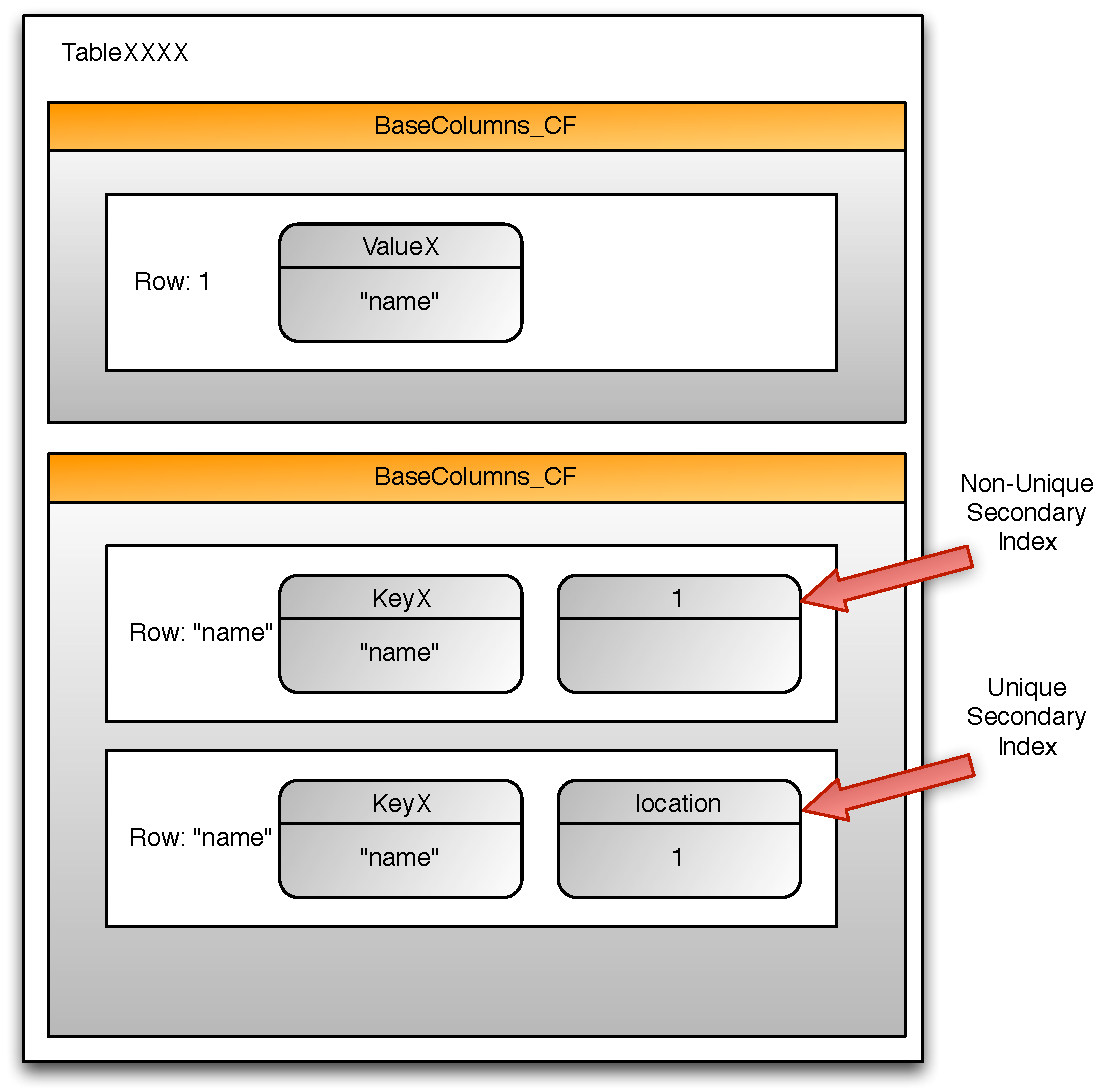
\includegraphics[width=0.7\textwidth]{images/mymodel}
  \end{center}
  \caption{Cassandra design to integrate with Derby}
  \label{fig:mymodel}
\end{figure}

\subsection{Records}
\label{sec:records}
A record, row or tuple all have the same meaning, they represent a container of values, typically in fixed number and indexed by names. In this specific context, they represent a structured data item that is stored in a database table. They are the assets we intend to maintain durable and consistent.

This means that when an insert or update action is performed one or more of these records must be created or updated, alongside with their corresponding indexes, as explained in section \ref{sec:derby_index}.

The various Derby operations that interact with the underlying data store had to be rewritten to be compliant with Cassandra. These operations encompass the creation and deletion of keyspaces, the insertion, replacement, fetching and deletion of rows, as well as the scans or range queries.

\subsubsection{Keyspace operations}
Since version 0.7 of Cassandra it is possible to alter keyspaces definitions on runtime, which allows us to create and delete them\footnote{keyspaces correspond to the relational tables and indexes, in our implementation}.

Therefore, when an \ac{sql} create table statement is issued, a keyspace is created, with the name defined according to the model and the replication factor and strategy coming from a configuration file. At the moment of creation of a keyspace, the respective column family is also created, taking into account if it is an index or not. The deletion is achieved through a call to the provided \emph{system\_drop\_keyspace} method.

While testing the system, we found some problems with these \emph{system} methods that allow the alteration of keyspaces. The main problem is that when a new keyspace is created, the method does not wait for the schema to agree. While this provides better performance since it does not block, it also means that if you try to do a query or an insert on that keyspace before the agreement of the schema, you will get an error that the system cannot come back from. We had to create our own method to wait for the schema agreement to avoid this errors.      

\subsubsection{Row operations}
The operations performed to a row are insert, replace, fetch and delete and as in the keyspaces they differ from indexes to normal records.

The insertion of a row consists on creating a column for each value, following the data model, and doing a batch update. For this operation the differences between indexes and normal records are not many, and are defined in section \ref{sec:data_model}. 

The replacement of a row only makes sense on normal records, since the indexes are managed internally. There are two main types of row replacements, when the primary key is going to change and when it is not. If the primary key changes and has a secondary or unique index, it is deleted and the new row is inserted (which will update the indexes), if it is not the new columns are added to Mutations and applied in a batch. Since this does not alter the primary it key, there is no need to update the indexes. In the first case, if the new row is not complete, the missing values must be fetched in order to complete it.

When fetching a row Derby gets the row for that index from which it extracts the location of the actual record and then does a second fetch, this time to the location pointed by the index. In figure \ref{fig:derbyindexes}, for example, Derby would fetch the row for index \emph{x} and get the location \emph{j}, from which it would get the \emph{info} from row \emph{j} in the records table.

This is fine for unique and secondary indexes, but as explained in the previous section, in the case of primary indexes there is no need for the creation of a specific row for the index, thus making this two fetches mechanism redundant. Since this redundancy meant an unnecessary access to the database, which could incur in a large overhead, this matter had to be addressed. 

The way this was solved was by storing in memory the whole row fetched in first place (through the index) and passing it on alongside with the actual record location. This allows for the tuple controller that is doing the fetch to use the information in memory, when it is available.

For the other types of indexes the location of the actual record must be fetched as well. In the case of unique indexes the column with name ``location'' is fetched and in the case of non-unique secondary indexes the remaining column has the location as its name. This location is added to the previously constructed row that is then validated and returned.

\begin{figure}[!h]
  \centering    
  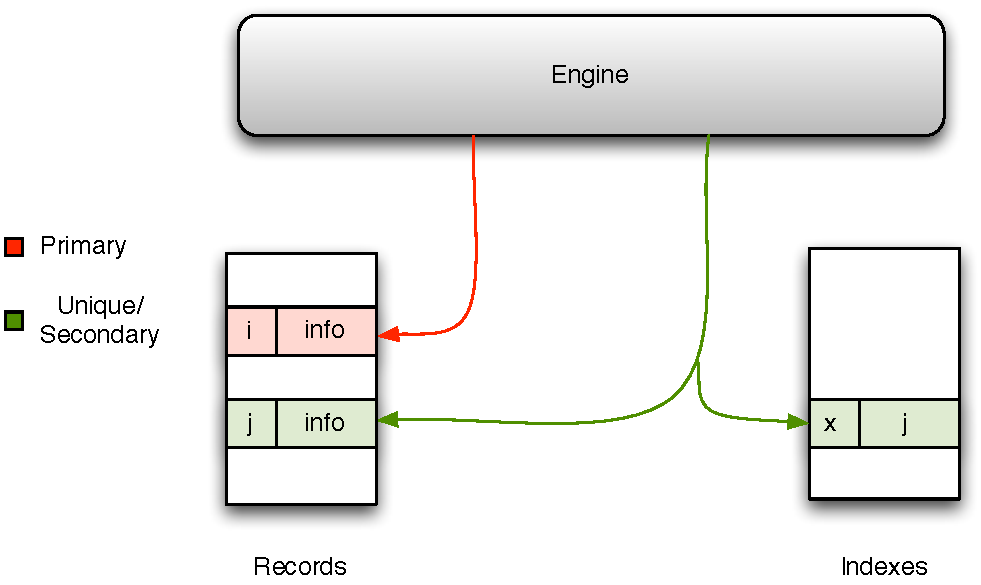
\includegraphics[width=0.9\textwidth]{images/derbyindexes}
  \caption{Derby Indexes}
  \label{fig:derbyindexes}
\end{figure}

In those cases where this optimization cannot be applied, what happens is that the necessary values (it is not mandatory to query for the entire row) are fetched and a Derby row is created and passed on.  

Rows are deleted with Cassandra's method \emph{remove}, which marks them as deleted for a certain time\footnote{this amount of time is called \emph{GCGraceSeconds} and is defined in cassandra's configuration file}. The reason a row is not deleted immediately is because of the fact that the \emph{remove} is actually performing a distributed delete, which means that some of the replicas may not receive the delete operation. In that case, if the data was to be deleted at once, when one of those replicas became available again it would treat the replicas that received the delete as having missed a write update, and repair them. That is why deleted data is replaced with a special Cassandra value called tombstone, that can later be propagated to the replicas that missed the initial remove request.

The reason for this tombstones to be available for a pre defined amount of time is that in a distributed system without a coordinator, it is impossible to know the moment when all the replicas are aware of the delete and it is safe to remove the tombstone. By default Cassandra waits ten days before removing them.


\subsection{Indexing}
\label{sec:derby_index}
Indexing is a way of sorting records on multiple fields. Creating an index on a field in a table creates another data structure with the field value, and a pointer to the primary record. 

The downside to indexing is that these indexes require additional space on the disk and processing time when inserting, updating or removing new data.

\subsubsection{Derby Indexes}
Along with the actual record handling classes, there are the ones responsible for the indexes, which can be of one of three types:

\begin{description}
	\item[Primary] Refers to primary keys. There can only be one per table and it must unambiguously match one, and only one, record.
	\item[Secondary] Secondary or Ordinary indexes are used to accelerate the process of finding a requested row's location by a given value in those cases where this value is not the primary key. 
	\item[Unique] Resemble ordinary (secondary) indexes, except they prevent duplicates from being added.	
\end{description} 

The creation of an index in our version of Derby depends on its type. 

When it is a primary index, Derby is informed about it (through a flag), but no actual index record is created in Cassandra, since in Cassandra it is mandatory for each row to have a key that in this case will be the primary key, and the rows are automatically indexed by that key (Fig. \ref{fig:derbyindexes}).

On the rest of the cases, an index is created according to the model defined in section \ref{sec:data_model}.

When fetching information that is indexed, Derby (as most \acp{rdbms}) first estimates the cost of fetching using the index or not, based on the number and size of the rows, and acts accordingly.

\subsubsection{Indexing in Cassandra}
Secondary indexes where introduced to Cassandra in version 0.7, they allow querying by value and can be built in the background automatically without blocking reads or writes. 

We have not used this, however, because there are still several limitations such as not being recommended for attributes with high cardinality, i.e. attributes that have a lot of unique values, and with these indexes only equality queries can be done, not range queries~\cite{secindexlimitations}.

In the cases where these limitations cannot be tolerated (such as ours) the documentation recommends using a separate column family and implement our own secondary index~\cite{secindex}. 

\subsection{Scans}
\label{sec:derby_scans}

A scan or range query, is the action triggered when the submitted query has inequality operators\footnote{$<$, $>$, $<=$ and $>=$} or uses the \emph{BETWEEN} or \emph{LIKE} operators.

In Derby, the range to which the query applies is passed on to the scan controller through a start and a stop key and a flag that defines if the range is inclusive or exclusive in either end. With this parameters, the controller fetches the needed rows to memory, validates each one and returns those which are valid.

\begin{figure}[!h]
  \centering    
  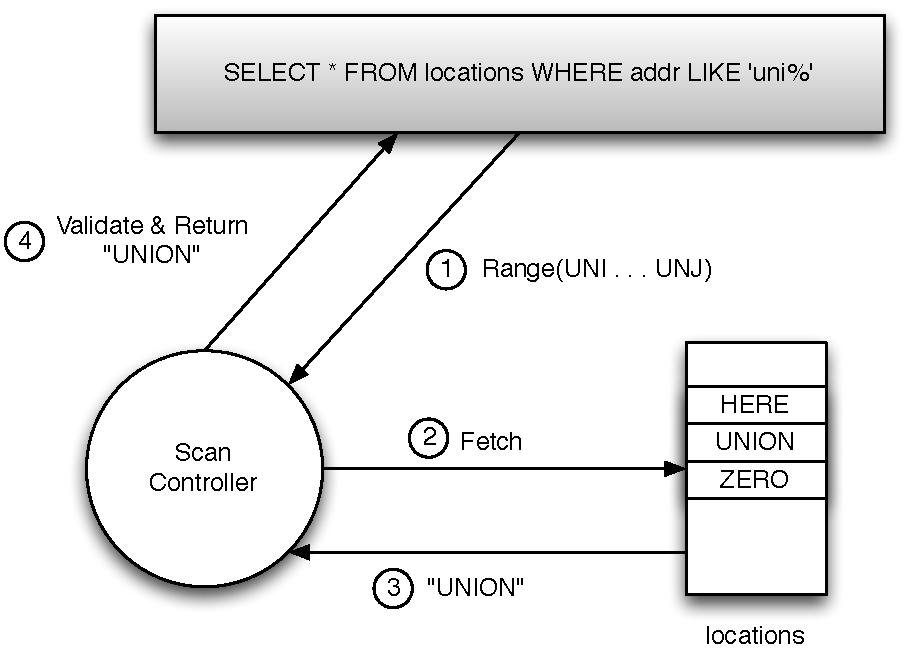
\includegraphics[width=0.7\textwidth]{images/likescan}
  \caption{Querying with \emph{LIKE}}
  \label{fig:likescan}
\end{figure}

As can be perceived from figure \ref{fig:likescan}, there are two assumptions that must be met in order for a \emph{LIKE} query to function properly.

\begin{enumerate}
	\item The keys must be ordered by their byte value, so that strings as well as integers and any other type of data are logically ordered\footnote{If they were ordered by their UTF-8 value, for example, the number 10 would be between 1 and 2, which means that a query for all records which have a value between 8 and 10, would return 2 records (8 and 9) instead of the expected 3 (8, 9 and 10)}.
	\item The encoding of the data types must be coherent throughout the application 
\end{enumerate}

The first assumption was met through the Ordered Partitioner that comes bundled with Cassandra, as was explained in section \ref{sec:partitioners}. The second one meant having classes to encode each type of data that Derby accepts (Integer, Float, String, DateTime, etc\ldots), as well as altering the way padding is applied to the strings that are received through a \emph{LIKE} query so that it becomes compliant with the way Cassandra stores its data. This has to be done because Cassandra does not allow for range queries on string prefixes. Take the example in figure \ref{fig:likescan}, for instance, the values in the range in step one have to be padded so that they have at least the same length as the value we are looking for, in this case \emph{UNION}. 

Both with normal records and indexes the primary method is \emph{fetchNext}, which returns the next row in the range. In the case of records this consists in getting the next row from the iterator and encoding the values to create a Derby row. 

\subsubsection{Scanning with indexes}

Performing a scan that involves fetching a row through an index is a bit more complex since the indexes can be of three types, which means doing things a little different for each of the types. 

When performing a scan that involves fetching a row through an index, Derby fetches row by row according to the mechanism in section \ref{sec:records}.

When performing scans in Cassandra there is one other detail to take in account, that is the fact that a column (or row) is only deleted after a certain amount of time, which means that some tombstones\footnote{special markers for columns that have been deleted} may be returned, these are known as range ghosts. Cassandra had a range query method that eliminated tombstones from the result set, but has been deprecated due to performance issues, therefore when iterating over the rows it is necessary to be aware that a row coming from a range query can have no columns at all if it has been deleted and is now a tombstone or just some of the columns have actual valid values.  




       \mbox{}
	\chapter{Fully Distributed Transactional Model}
	\label{chap:fdtm}
       With these changes to Derby we have gained scalability, fault and partition tolerance and kept durability. This of course came with the cost of loosing atomicity\footnote{Cassandra provides atomicity at the row level, which is fine when doing separate inserts at a time, but is not good enough when performing batch inserts, in our model}, isolation and consistency (we have eventual consistency). 

In practical terms this means that transactions are not be possible with this system. To overcome these limitations we built a distributed transaction system that takes advantage of Cassandra's peer to peer architecture with the exception of a Zookeeper cluster to manage the locks. This cluster and why it is not a big limitation to the overall performance of the system are further explained in section \todo{secção do Zk e Cages}.

\section{Algorithm}
The adopted algorithm (Fig. \todo{algoritmo}) combines a mechanism of locks and a write ahead log with Cassandra's provided atomicity and idempotent operations.

\missingfigure{O algoritmo transaccional}

\section{Locks}
Before the actual transaction can start, it must acquire the locks for the rows (or entire tables) it is going to use. These locks are kept in a Zookeeper cluster, using a library called Cages.

The actual lock mechanism works by first asking for a lock for the table called \emph{any\_or\_all}, when attempting to lock the entire table this is a write lock, otherwise it is a read lock. In the second case there is a second step of asking for locks on the rows we need, since there can be many threads with read locks on the same table at the same time. This means that all threads can pass on to ask for locks in the rows, unless there is another wanting to lock the whole table. 

Each lock is represented by a Path class, that encapsulates the path to lock as well as its type (table lock or not) and provides the necessary primitives to work with it. 

Still this mechanism is not enough because it does not prevent deadlocks\footnote{If two threads want locks A and B, and one of them gets A and the other B, they will both be waiting on the other, which is the definition of a deadlock}. In order to do this, there has to be a globally accorded way of ordering the paths of the locks, for this we first compare the nesting of the path (table locks are less nested and therefore are sorted first), then we compare the actual name of the table\footnote{using Java strings default compareTo method} and at last, in the case of rows of the same table, we compare the name of the row. This comparison in done with a Comparator class, which provides a way to change the way paths are compared without changing the code of the actual system.

\subsection{Cages}
\todo[inline]{Falar do cages e como funciona}

\subsection{Zookeeper}
\todo[inline]{Falar um bocadinho de zookeeper, com principal enfase nos observers}



      
   	   \mbox{}
    
    \chapter{Results and Performance Analysis}
       In order to evaluate the impact of having Cassandra as a datastore for \ac{sql} queries as opposed to running them on Derby, and to measure the overhead of using our transactional system we ran three different types of tests, the TPC-W benchmark, Yahoo! Cloud Serving Benchmark and scaling out process. This chapter details those tests and consequent results. 

\section{Testing Environment}
The tests were ran on HP computers with an Intel(R) Core(TM)2 CPU 6400 - 2.13 GHz processor, two Gigabytes of RAM and a SATA (7200 RPM) hard drive. The multiple machines are connected by LAN to a 1GB/s switch and run a Linux operating system, more specifically an Ubuntu Server, 2.6.31-1 kernel and an ext4 filesystem. 
All the test were run using between 2 and 8 of these machines according to the specific needs of each test. 

\section{TPC-W Benchmark}
The TPC-W benchmark specifies an e-commerce workload that simulates customers browsing, ordering and buying products from a website. The proposed solution for this benchmark is a number of servers (Web Servers, Web Caches, Image Servers and Database Server) working in concert to provide an e-commerce solution that is very similar to how an actual website performing this kind of business would operate. 

This benchmark tests various system components that are associated with such an environment, such as~\cite{tpcw}:

\begin{itemize}
	\item The simultaneous execution of multiple transaction types that span a breadth of complexity
	\item Databases consisting of many tables with a wide variety of sizes, attributes, and relationships
	\item Transaction integrity (ACID properties)
	\item Contention on data access and update
\end{itemize}

The transaction in TPC-W can be divided into two main sets, the write operations such as adding a product to the shopping cart or ordering a product and the read operations that simulate the search of products by title, author or subject or to ask for the more recent items or the ones that have sold the most. The first set of operations is called \textbf{order} and the second \textbf{browse}.

The variation of percentage of each of these sets defines three different mixes for the benchmark:

\begin{description}
	\item[Browsing] 95\% Browsing and 5\% Ordering
	\item[Shopping] 80\% Browsing and 20\% Ordering
	\item[Ordering] 50\% Browsing and 50\% Ordering
\end{description}

Most use cases where \acp{vlsd} are used perform a lot of reads and few writes (browsing through a website) therefore, we chose the Browsing mix to perform our tests.

The configurable parameters are the numbers of \acp{eb} which represent the number of clients, and the number of items in the system, all the other parameters such as the number of customer, addresses, authors or orders, are relative to these ones.

In order to compare our implementation with and without the transactional guarantees with the standard Derby Client/Server configuration, we used one machine to serve as Client, Database Server and Web Server for all three cases. For our implementation we also used one machine as a Cassandra node and another one as a Zookeeper node for the transactional system. We tested the system with 1000 items and a varying number of clients, ranging from 10 to 100 with the results for throughput and latency show in figure \ref{fig:tpm10} and \ref{fig:lat10}, respectively.

\begin{figure}[!ht]
  \begin{center}\subfigure[Throughput]{\label{fig:tpm10}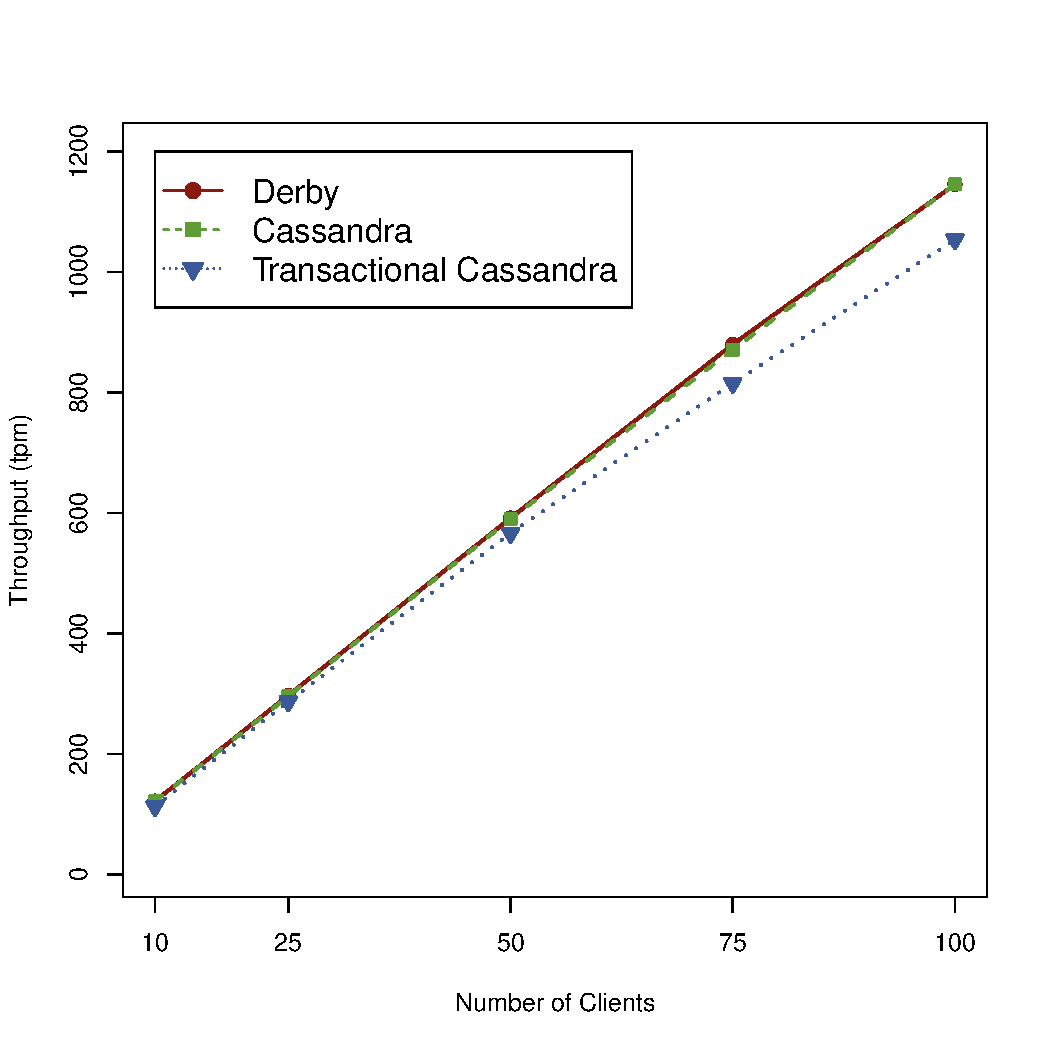
\includegraphics[width=0.7\textwidth]{images/tpcw_tpm.pdf}}\end{center}
  \begin{center}\subfigure[Latency]{\label{fig:lat10}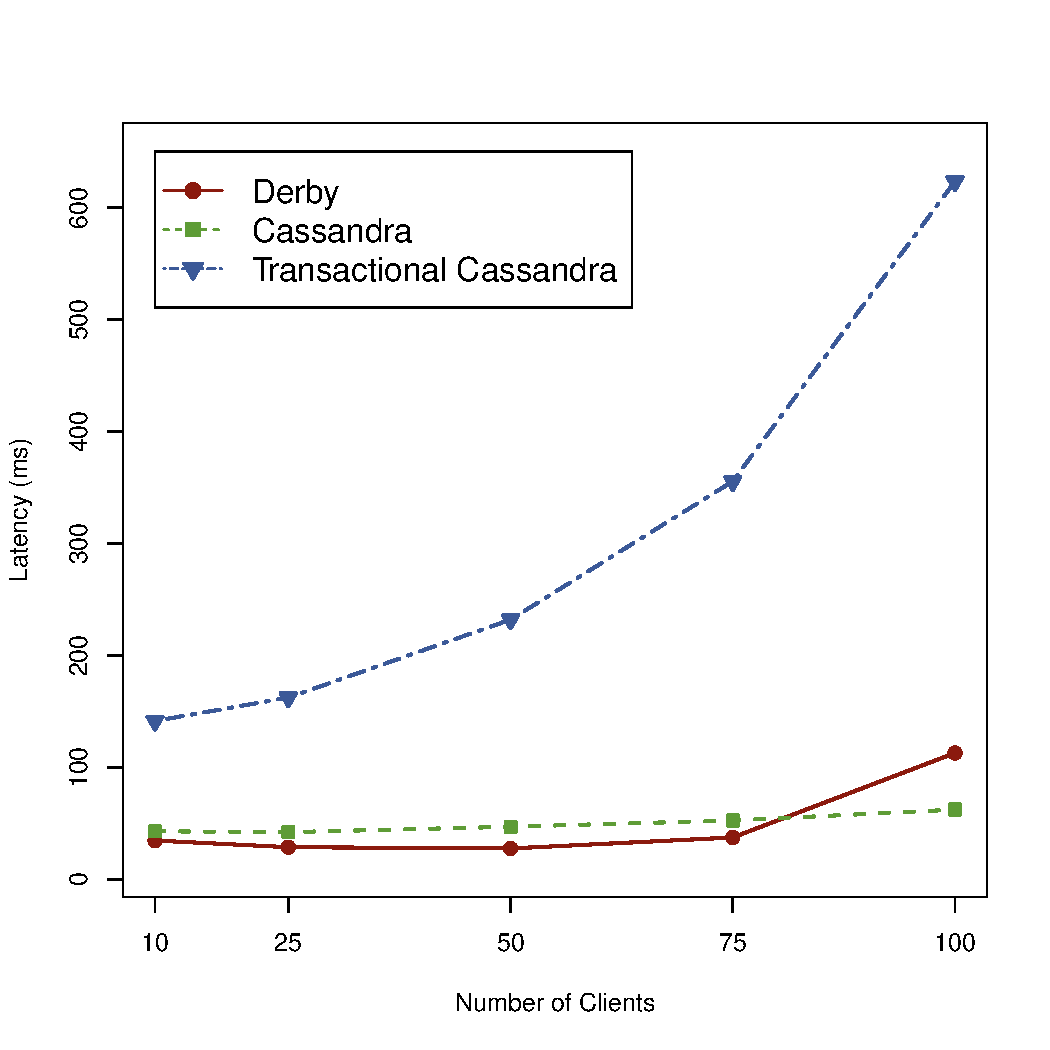
\includegraphics[width=0.7\textwidth]{images/tpcw_lat.pdf}}\end{center}
  \label{fig:tpcw10}
  \caption{Results of running TPC-W with different number of clients}
\end{figure}
 

\section{Yahoo! Cloud Serving Benchmark}

\ac{ycsb} is a framework presented by Yahoo!\footnote{\url{www.yahoo.com}} with the goal of facilitating performance comparisons of the new generation of cloud data serving systems. It focuses on \emph{serving} systems, which are systems that provide online read/write access to data such as Cassandra, as opposed to batch or analytical systems such as Hadoop~\cite{Cooper:2010:BCS:1807128.1807152}.

The workloads in the core package of \ac{ycsb} are a variation of the same application type. The application has one table of records each with \textbf{F} fields and identified by a primary key which is a string like ``user12345''. Each field is named \emph{field0}, \emph{field1}, and so on and has a random string of ASCII characters of length \textbf{L} as value. The operations against the data store are randomly chosen to be one of the following~\cite{Cooper:2010:BCS:1807128.1807152}:

\begin{description}
	\item[Insert] Insert a new record
	\item[Update] Update a record by replacing the value of multiple fields
	\item[Read] Read a record, either one randomly chosen field or all fields
	\item[Scan] Scan records in order, starting at a randomly chosen record key. The number of records to scan is randomly chosen from a configurable distribution (Uniform, Zipfian, Latest or Multinomial)
\end{description}

\ac{ycsb} also provides a tool called \ac{ycsb} Client to execute the benchmark, this tool has 5 workloads with different configurations. We introduced a new operation called multiupdate that performs updates on multiple rows, and to accommodate it we also created our own workload with 95\% reads, of which 80\% are actual read operations and 15\% are scans, and 5\% multiupdates.

For this test we used one machine running Cassandra for both the normal and transactional setting alongside with one zookeeper node for the latter. The results are shown for the scan operation are shown in figure \ref{fig:ycsb_scan}, for the read operation in figure \ref{fig:ycsb_read} and for the multiupdate in figure \ref{fig:ycsb_update}.

\begin{figure}[!ht]
  \subfigure[Scan]{\label{fig:ycsb_scan}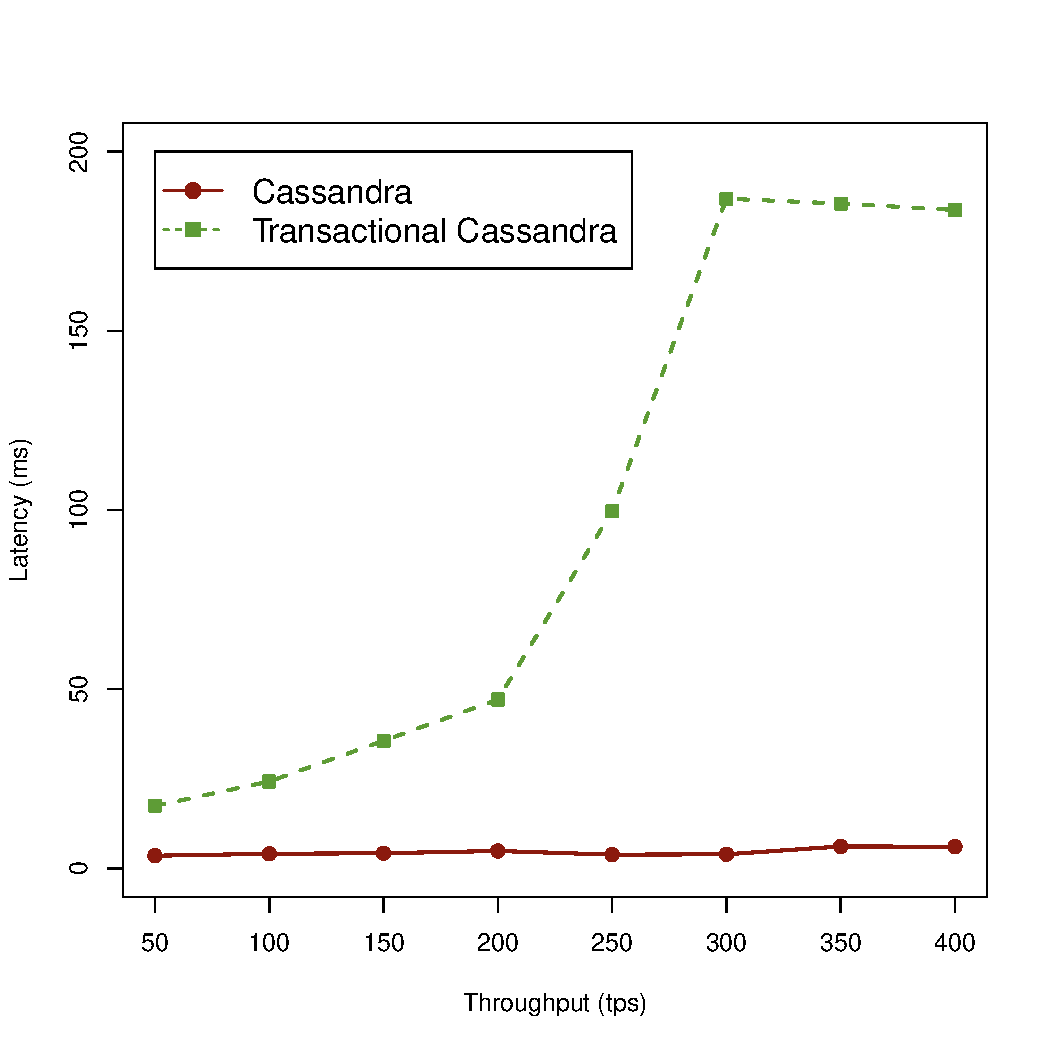
\includegraphics[width=0.5\textwidth]{images/ycsb_scan.pdf}}
  \subfigure[Read]{\label{fig:ycsb_read}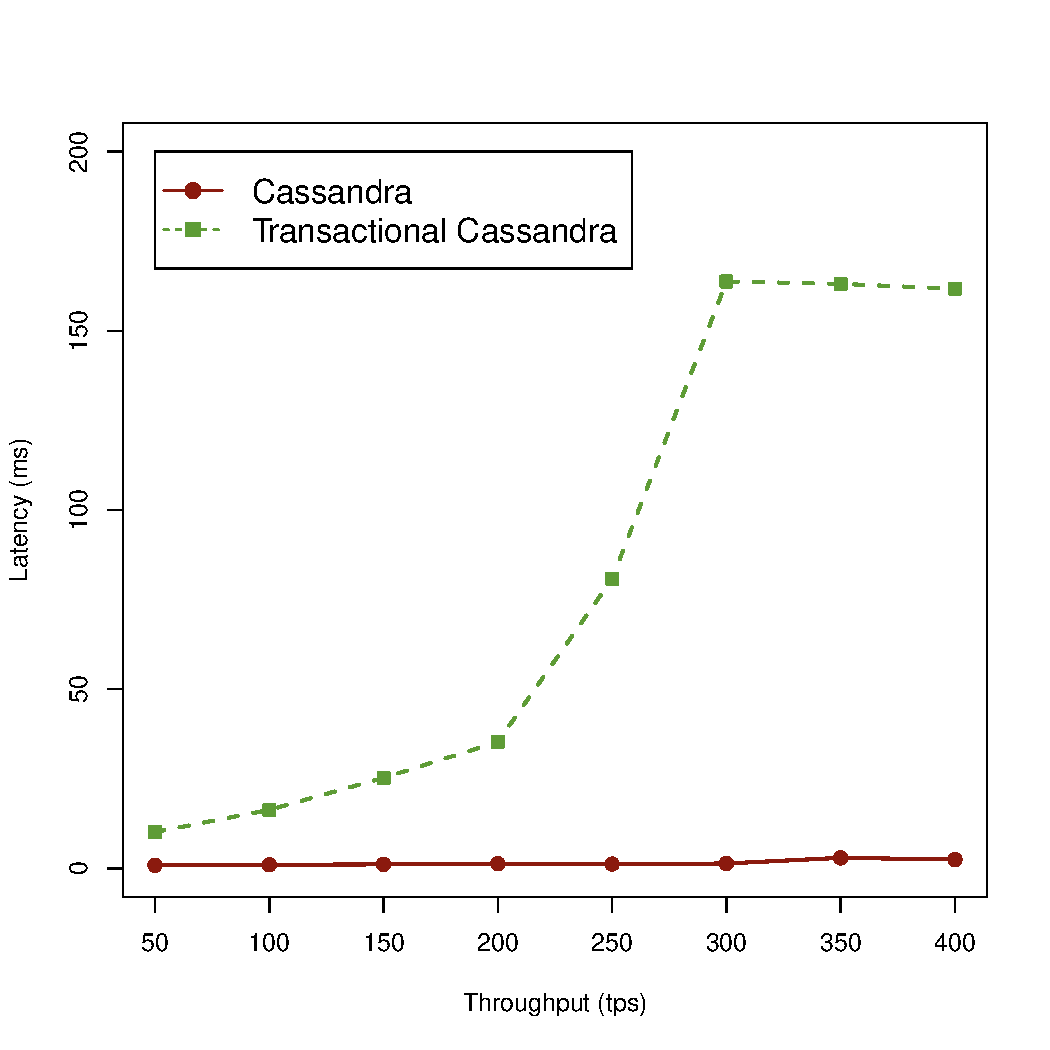
\includegraphics[width=0.5\textwidth]{images/ycsb_read.pdf}}
  \begin{center}\subfigure[Multiupdate]{\label{fig:ycsb_update}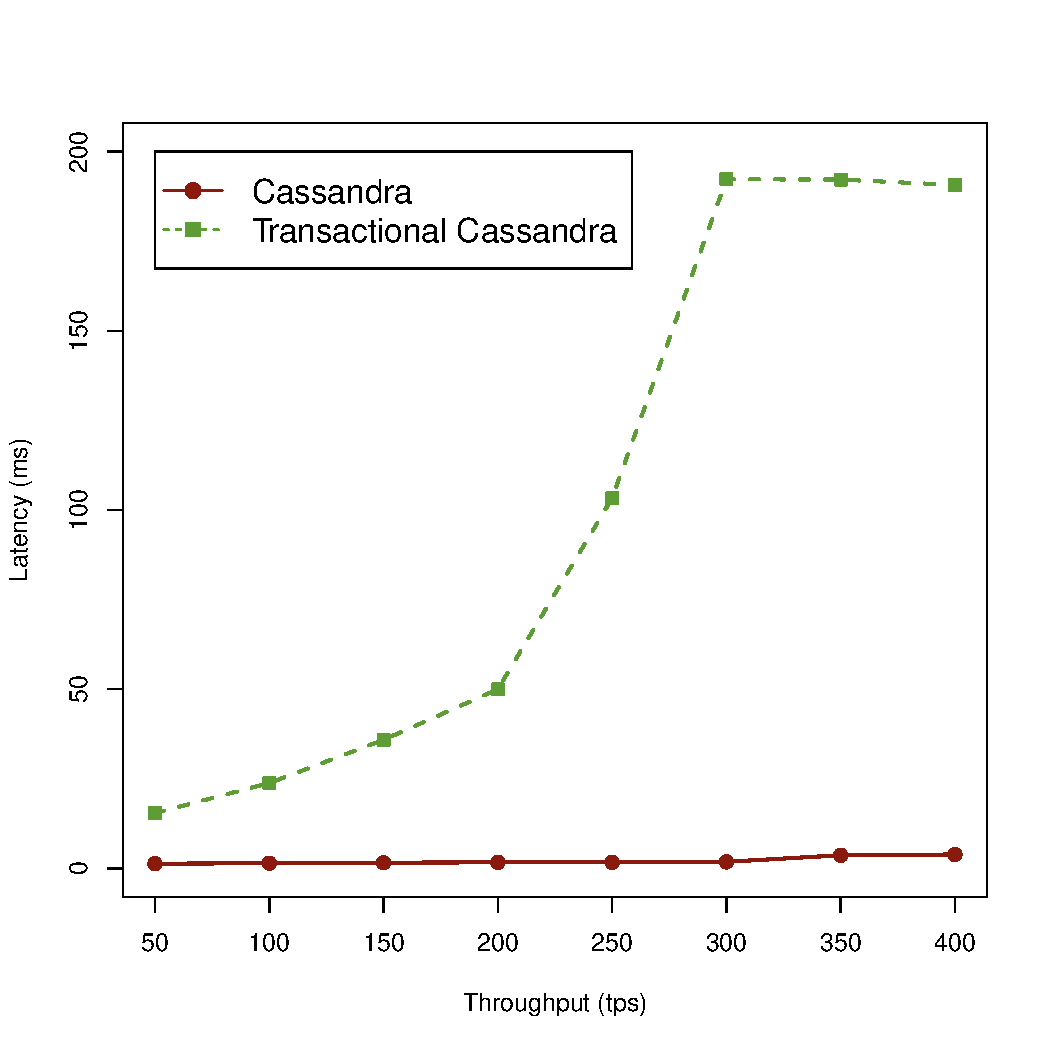
\includegraphics[width=0.5\textwidth]{images/ycsb_update.pdf}}\end{center}
  \label{fig:ycsb}
  \caption{Results of running YCSB with different expected throughput}
\end{figure}


\section{Scaling out}

So that we could better understand how the number of nodes in the cluster affected the system we tested its performance with 100 clients and 1000 items with the number of Cassandra nodes ranging from 1 to 5.  



   	   \mbox{}	
	%	\newpage
		\thispagestyle{plain}
		\mbox{}
    \chapter{Related Work}
       Our work spans over several areas such as altering the processor part of an \ac{sql} query engine and distributed transactions. There is also some work on high level interfaces for \acp{vlsd} that we find is worth mentioning.

\section{SQL over Memory}
The idea of patching Derby so that the data is stored in a different way than normal is not entirely new and was firstly introduced by Knut Magne Solem~\cite{derbyPatch}. In his approach all the tables whose name began with \emph{MEM} were stored in memory, as opposed to our approach which stores in Cassandra all the tables whose name starts with \emph{TUPLE}.

\section{Distributed Transactions}

Transactions become difficult under heavy load. When you first attempt to horizontally scale a relational database, making it distributed, you must now account for distributed transactions, where the transaction isn’t simply operating inside a single table or a single database, but is spread across multiple systems. In order to continue to honor the ACID properties of transactions, you need a transaction manager to orchestrate across the multiple nodes.

There are many leader election algorithms but they all have the same input and output. At the beginning there is a set of nodes in a network, unaware of which of them is the leader, after the protocol they all recognize a particular, unique node as the leader.

Assuming that the leader is already elected, a simple way to complete a distributed transaction in an atomic manner is for the coordinator to communicate the commit or abort request to all of the participants in the transaction and keep repeating the request until all of them have acknowledged that they have carried it out. This is called one-phase commit protocol~\cite{coulouris2005distributed} and is inadequate because it does not allow a server to make a unilateral decision to abort a transaction. 

\subsubsection{Two-phase commit protocol}

The two-phase commit protocol is designed to allow any participant to abort its part of a transaction which, by the atomicity requirement, means the whole transaction must be aborted. 

In the first phase of the protocol the coordinator asks all of the participants if they are prepared to commit and in the second it tells them to commit/abort the transaction. Once a participant has voted to commit a transaction it is not allowed to abort it, therefore a participant must before make sure it will be able to carry out its part of the protocol, before committing to it. 

\begin{table}[h!]
\centering
  \begin{tabular}{  l  p{8cm}}
	\toprule
	Operation & Description\\
    \midrule
    \emph{canCommit?(trans) $\rightarrow$ Yes/No} & Coordinator asks if it can commit a transaction. Participant replies with vote.\\  
    \emph{doCommit(trans)} & Coordinator tells participant to commit its part.\\
    \emph{doAbort(trans)} & Coordinator tells participant to abort its part.\\
    \emph{haveCommited(trans,participant)} & Participant tells the coordinator it has commited.\\
    \emph{getDecision(trans) $\rightarrow$ Yes/No} & Participant asks for decision after it has voted. Used to recover from server crashes or delayed messages.\\
	\bottomrule
  \end{tabular}

\caption{Operations for two-phase commit protocol (based on \cite{coulouris2005distributed})}
\label{tab:2pc_ops}
\end{table}

Using the operations defined in table \ref{tab:2pc_ops}, a successful run of the protocol with one coordinator and one participant is as shown by figure \ref{fig:2pc_run}.

\begin{figure}[htb]
  \begin{center}
    \leavevmode
    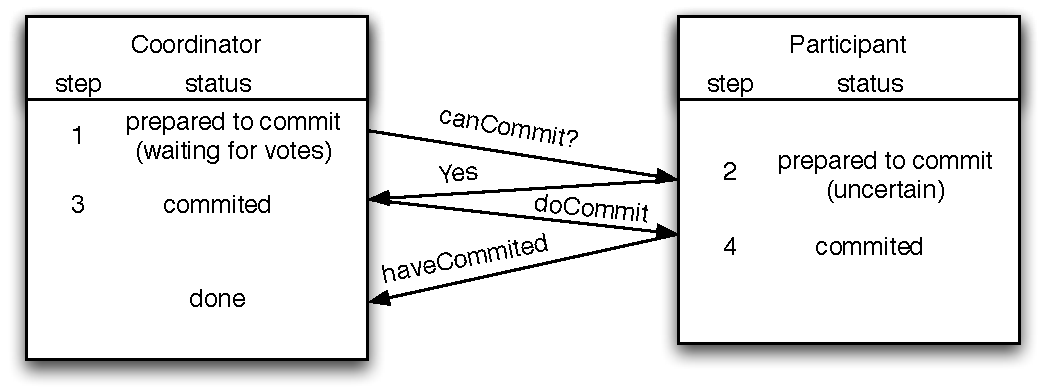
\includegraphics[width=0.9\textwidth]{images/2pc}
  \end{center}
  \caption{Two-phase commit successful run\cite{coulouris2005distributed}}
  \label{fig:2pc_run}
\end{figure}

\subsection{CloudTPS}
One particular implementation of distributed transactions, i.e. offers transactional guarantees (ACID) over a \ac{vlsd}, is CloudTPS~\cite{cloudTPS} which chooses to provide strong consistency at the cost of the possibility of becoming unavailable when facing network partition. In order to provide full transactional guarantees it introduces the concept of \acp{ltm} which are various parts of a transaction manager called transaction processing system, each of them is responsible for a part of the data and for processing certain parts of the transaction.

Since a transactional system must maintain the ACID properties even in the case of server failures, the data items and transactions state are replicated to multiple \acp{ltm} and consistent data snapshots are periodically checkpointed to the cloud storage system in order to guarantee the durability of each transaction.

The client can submit a transaction to any \ac{ltm} that is responsible for one of the accessed item, which then acts as the coordinator of the transaction across all \acp{ltm} responsible for the data items needed by the transaction, which is implemented using the two-phase commit protocol where the other \acp{ltm} are the participants.


\section{High Level Interfaces for a \ac{vlsd}}
\acp{vlsd}' query interfaces are in general very low level and do not conform to any type of standard which, as has been pointed out, leads to many problems including portability of code. There have been several projects that have proposed different high level interfaces for the \acp{vlsd} in order to mitigate this problem. 

\subsection{Object Mapper}

Using object mapping tools in order to allow to bypass the lower level interfaces of Cassandra is one the possible approaches, and is the one taken by the Cassandra Object Mapper~\cite{Pi}. 

In this project the user has at its disposal generic object interfaces like JPA and JDO that allow him to use the underlying database in an almost transparent way, which greatly simplifies the reading and writing of data. This transparency also brings the advantage of aiding in the migration of existent solutions and allowing the mix of different types of data stores under the same code base.  

The underlying store can be a Cassandra cluster which will, therefore, be available to the user through one of those interfaces with all their expressiveness and features, such as JDO class annotations.

One of the downsides of this solution is that it offer no transactional guarantees and therefore some of features that would be expected in this kind of the tool are thereby unavailable to the user. 

\subsection{Hive}
Hive~\cite{Thusoo:2009:HWS:1687553.1687609} was initially developed at Facebook and is now an Apache project. It is built on top of Apache Hadoop and facilitates querying and managing of large datasets in distributed storage by providing a mechanism to impose structure on a variety of data formats and access to files stored directly in Apache HDFS or in other storage systems. 

It defines a simple SQL-like query language, called \emph{HiveQL}, whose queries are executed via MapReduce with the particularity that there is no specific data format, it works on Thrift and allows for the creation of specialized data formats. Also, it enables users to plug in custom map-reduce scripts into queries.

Hive is not designed for online transaction processing and it is best used for batch jobs over large sets of append-only data since what it values most is scalability, extensibility, fault-tolerance and a loose coupling between it and its input formats. 

\subsection{\acl{cql}}

The \ac{cql} \cite{cql}, is a really novel approach to this matter, being developed by Eric Evans. His idea, is to develop a \ac{sql} like query language on top of Cassandra, bypassing an \ac{sql} interpreter altogether at the expense of not being compatible with actual \ac{sql}  code. Still, this would allow for much faster adaptation to Cassandra, for people with relational background. 

\ac{cql} has been released with Cassandra new stable version (0.8), and a select query will look somewhat like this \cite{cqlSelect}:

\begin{center}
\begin{verbatim}
    SELECT (FROM)? <CF> [USING CONSISTENCY.<LVL>] WHERE 
       <EXPRESSION> [ROWLIMIT X] [COLLIMIT Y] [ASC|DESC]
\end{verbatim}
\end{center}

And would be replacing a lot of old methods for retrieving data as \emph{get()}, \emph{get\_slice()}, \emph{get\_range\_slices()}, and so on.	

At the time of writing there are still some features to be implemented~\cite{cqlbbw}, such as \emph{ALTER} and prepared statements and some SQL features that will not be implemented at all, as joins and update\footnote{Since cassandra 0.7 the updates are viewed as a special case of insert}.

   	\mbox{}	
   \chapter{Conclusions}
   	\label{sec:conclusion}
The lack of a standard querying \ac{api} and the relaxation in consistency alongside with the provided high availability, scalability and increased performance in certain use cases, makes \acp{vlsd} a thriving field of study and interest amongst the distributed systems community. However, all this properties also make it hard to migrate code from existing relational databases both because of the different interfaces and the lack of transactional guarantees so important in many scenarios.

With this work, we showed that it is possible to integrate a \ac{vlsd} with a \ac{rdbms} to the extent of providing an \ac{sql} interface for the former. In this context, the problems of such integration are described and a mapping of operations are proposed between DerbyDB and Cassandra.

In order to provide the transactional (ACID) guarantees, we propose a distributed transactions library based on a \ac{wal} mechanism and taking advantage of some of the guarantees of the actual \ac{vlsd}, in this case Cassandra. This library and how it can be integrated with the rest of the system is fully explained.

The tests performed show that ...  

Our system is modular and can be divided into four main parts:
\begin{description}
	\item[Applications (clients)] There can be multiple clients connect to the system
	\item[Core] Composed by the query engine and our abstraction layer, which contains the transactional system
	\item[Storage] This can be a cluster of multiple machines
	\item[Transactional Metadata] The metadata of the locking mechanism is stored in a Zookeeper cluster that can also be composed multiple machines
\end{description}

This modular approach combined with the provided functionality and new ideas makes this work a viable way to integrate legacy \ac{sql} code with a \ac{vlsd}. 

\section{Future Work}
The presented system solves the problems of providing an \ac{sql} interface and transactional functionality over a \ac{vlsd}. It has, however, certain limitations and some areas that can be further explored.

The main limitation of the system is that it does not provide snapshot isolation, this property comes directly from the fact that Cassandra does not allow multiple versions of a column.

This system is built specifically for the case of Derby and Cassandra and the transactional system is specially linked with Cassandra. An area to be explored would be building such a system for other \acp{vlsd} and if possible build a generic transactional system for most, if not all, \acp{vlsd}. 
   	\newpage
   	\thispagestyle{plain}
   	\mbox{}

	\bibliographystyle{alpha}
%	\bibliographystyle{abbrv}
	\cleardoublepage
	\renewcommand\bibname{References}
	%\addcontentsline{toc}{chapter}{References}
	\bibliography{references}
	
	\appendix
		%\chapter{Additional Results}
		%	\section{MySQL Replication}

\subsection{Master and Multiples Slaves}

\begin{figure}[h!]
\centering    
\includegraphics[width=1\textwidth]{images/mms_semproxy/tt0_new/histo.pdf}
\caption{Replication delay values for Master and Multiple Slaves topology (no think-time)}
\end{figure}

\begin{figure}[h!]
\centering    
\includegraphics[width=1\textwidth]{images/mms_semproxy/tt03/histo.pdf}
\caption{Replication delay values for Master and Multiple Slaves topology (one-third of think-time)}
\end{figure}

\clearpage

\subsection{Chain}

\begin{figure}[h!]
\centering    
\includegraphics[width=1\textwidth]{images/chain/tt0_new/histo.pdf}
\caption{Replication delay values for Chain topology (no think-time)}
\end{figure}

\begin{figure}[h!]
\centering    
\includegraphics[width=1\textwidth]{images/chain/tt03/histo.pdf}
\caption{Replication delay values for Chain topology (one-third of think-time)}
\end{figure}

\clearpage

\section{Proxy Spread Plugins - Active Replication}

\subsection{FIFO Messages}

\begin{figure}[h!]
\centering    
\includegraphics[width=1\textwidth]{images/mms_comproxy_fifo/tt03/histo.pdf}
\caption{Replication delay values for active replication with Proxy Spread plugins with FIFO messages (one-third of think-time)}
\end{figure}

\clearpage


\subsubsection{Varying number of replicas}

\begin{figure}[h!]
\centering    
\includegraphics[width=1\textwidth]{images/mms_comproxy_fifo_varrepl/tt03_2repl/histo.pdf}
\caption{Replication delay values for active replication with Proxy Spread plugins with FIFO messages (one-third of think-time, two replicas)}
\end{figure}

\begin{figure}[h!]
\centering 
\includegraphics[width=1\textwidth]{images/mms_comproxy_fifo_varrepl/tt03_4repl/histo.pdf}
\caption{Replication delay values for active replication with Proxy Spread plugins with FIFO messages (one-third of think-time, four replicas)}
\end{figure}

\clearpage

\subsection{AGREED Messages}

\begin{figure}[h!]
\centering    
\includegraphics[width=1\textwidth]{images/mms_comproxy_agreed/tt03/histo.pdf}
\caption{Replication delay values for active replication with Proxy Spread plugins with AGREED messages (one-third of think-time)}
\end{figure}

\clearpage

\subsubsection{Varying number of replicas}

\begin{figure}[h!]
\centering    
\includegraphics[width=1\textwidth]{images/mms_comproxy_agreed_varrepl/tt03_2repl/histo.pdf}
\caption{Replication delay values for active replication with Proxy Spread plugins with AGREED messages (one-third of think-time, two replicas)}
\end{figure}

\begin{figure}[h!]
\centering    
\includegraphics[width=1\textwidth]{images/mms_comproxy_agreed_varrepl/tt03_4repl/histo.pdf}
\caption{Replication delay values for active replication with Proxy Spread plugins with AGREED messages (one-third of think-time, four replicas)}
\end{figure}
		%	
		\chapter{Code}
		    \label{app:code}
			\section{Lua Script to use on Proxy Spread Master Plugin}

\verb+ mysql-proxy --plugins=proxyspread_master --proxyspread-lua-script=spreadrepl.lua +\verb

\vspace{10mm}

\Large \textbf{spreadrepl.lua}\\
\small

\begin{lstlisting}
function read_query(packet)

	query = string.sub(packet, 2)
	
	--print("Seen the query: " .. query)	

	spread_send_msg(query)

end
\end{lstlisting}

\end{document}